\documentclass[oneside, 12pt]{book}
\usepackage[polish]{babel}
\usepackage{geometry}
\usepackage{lipsum}
\usepackage{nameref}
\usepackage{polski}
\usepackage[utf8]{inputenc}
\usepackage{setspace}
\usepackage[export]{adjustbox}
\usepackage{biblatex}
\usepackage{titlesec}
\usepackage{csquotes}
\usepackage{float}

\usepackage[table]{xcolor} % For cell colors
\usepackage{array} % For table alignment
\usepackage{colortbl} % For color in tables
\usepackage{booktabs} % For better-looking tables
\usepackage{svg}

\usepackage[pdfsubject={Pielat K.: Analysis of the Influence of Acoustic
Parameters and Lyrics on the Characteristics of Music Tracks Using AI Methods},
pdfauthor={Pielat K.},
pdftitle={Pielat K.: Analysis of the Influence of Acoustic Parameters and
Lyrics on the Characteristics of Music Tracks Using AI Methods},
pdfkeywords={musical analysis; nlp; acoustic analysis}]{hyperref}
\usepackage{tabularray}

\addto\captionspolish{
  \renewcommand{\figurename}{Figure}
}

\addto\captionspolish{
  \renewcommand{\tablename}{Table}
}

\addto\captionspolish{
  \renewcommand{\contentsname}{Table of Contents}
}

\setcounter{tocdepth}{3}
\setcounter{secnumdepth}{3}

\addbibresource{bibliography.bib}

\titleformat{\chapter}[block]
  {\normalfont\huge\bfseries}{\thechapter.}{1em}{\Huge}

\titlespacing*{\chapter}{0pt}{50pt}{40pt}

\geometry{
    top=1in,
    bottom=1in,
    outer=1in,
    inner=1in,
}

\pagestyle{plain} %Numeracja na dole

\linespread{1.5} % Interlinia 1.5

\setlength{\parindent}{1.25cm} % Wcięcie akapitu 1.25cm

\begin{document}
\thispagestyle{empty}

% Informacje na stronę tytułową
\newcommand{\autor}{\fontfamily{qhv}\fontshape{n}\selectfont\LARGE\bfseries
Krystian Pielat}
%
\newcommand{\album}{\fontfamily{qhv}\fontshape{n}\selectfont
143007}

\newcommand{\pltitle}{\fontfamily{qhv}\fontshape{n}\selectfont\Large\bfseries
Analiza wpływu parametrów akustycznych i tekstów na charakterystykę utworów muzycznych z wykorzystaniem metod sztucznej inteligencji}
\newcommand{\engtitle}{\fontfamily{qhv}\fontshape{n}\selectfont\Large\bfseries
 Analysis of the Influence of Acoustic Parameters and Lyrics on the Characteristics of Music Tracks Using AI Methods}
\newcommand{\level}{\fontfamily{qhv}\fontshape{n}\selectfont\Large
inżynierska} %jeśli magisterka to trzeba sobie przystosować pamiętając o specjalności
\newcommand{\kierunek}{\fontfamily{qhv}\fontshape{n}\selectfont\Large
Informatyka}
%
\newcommand{\promotor}{\fontfamily{qhv}\fontshape{n}\selectfont\large\bfseries
dr inż. Daniela Grzonki}
\newcommand{\spec}{\fontfamily{qhv}\fontshape{n}\selectfont\Large\bfseries
Brak}
\newcommand{\rok}{\fontfamily{qhv}\fontshape{n}\selectfont
2024}

% Strona tytułowa
\begin{titlepage}
\thispagestyle{empty}
\vspace*{1ex}
\fontfamily{qhv}\fontshape{n}\selectfont
\hspace{-3.5em}\parbox{0.15\textwidth}{
\includegraphics[height=0.15\textwidth]{logo_pk/logoPK.png}}
\parbox[c]{0.7\textwidth}
{\centering
\Large
{\bfseries Politechnika Krakowska}\\
{\bfseries im. Tadeusza Kościuszki}\\

\smallskip

\Large Wydział Informatyki i Telekomunikacji}\hspace{0.3em}
 \parbox{0.2\textwidth}{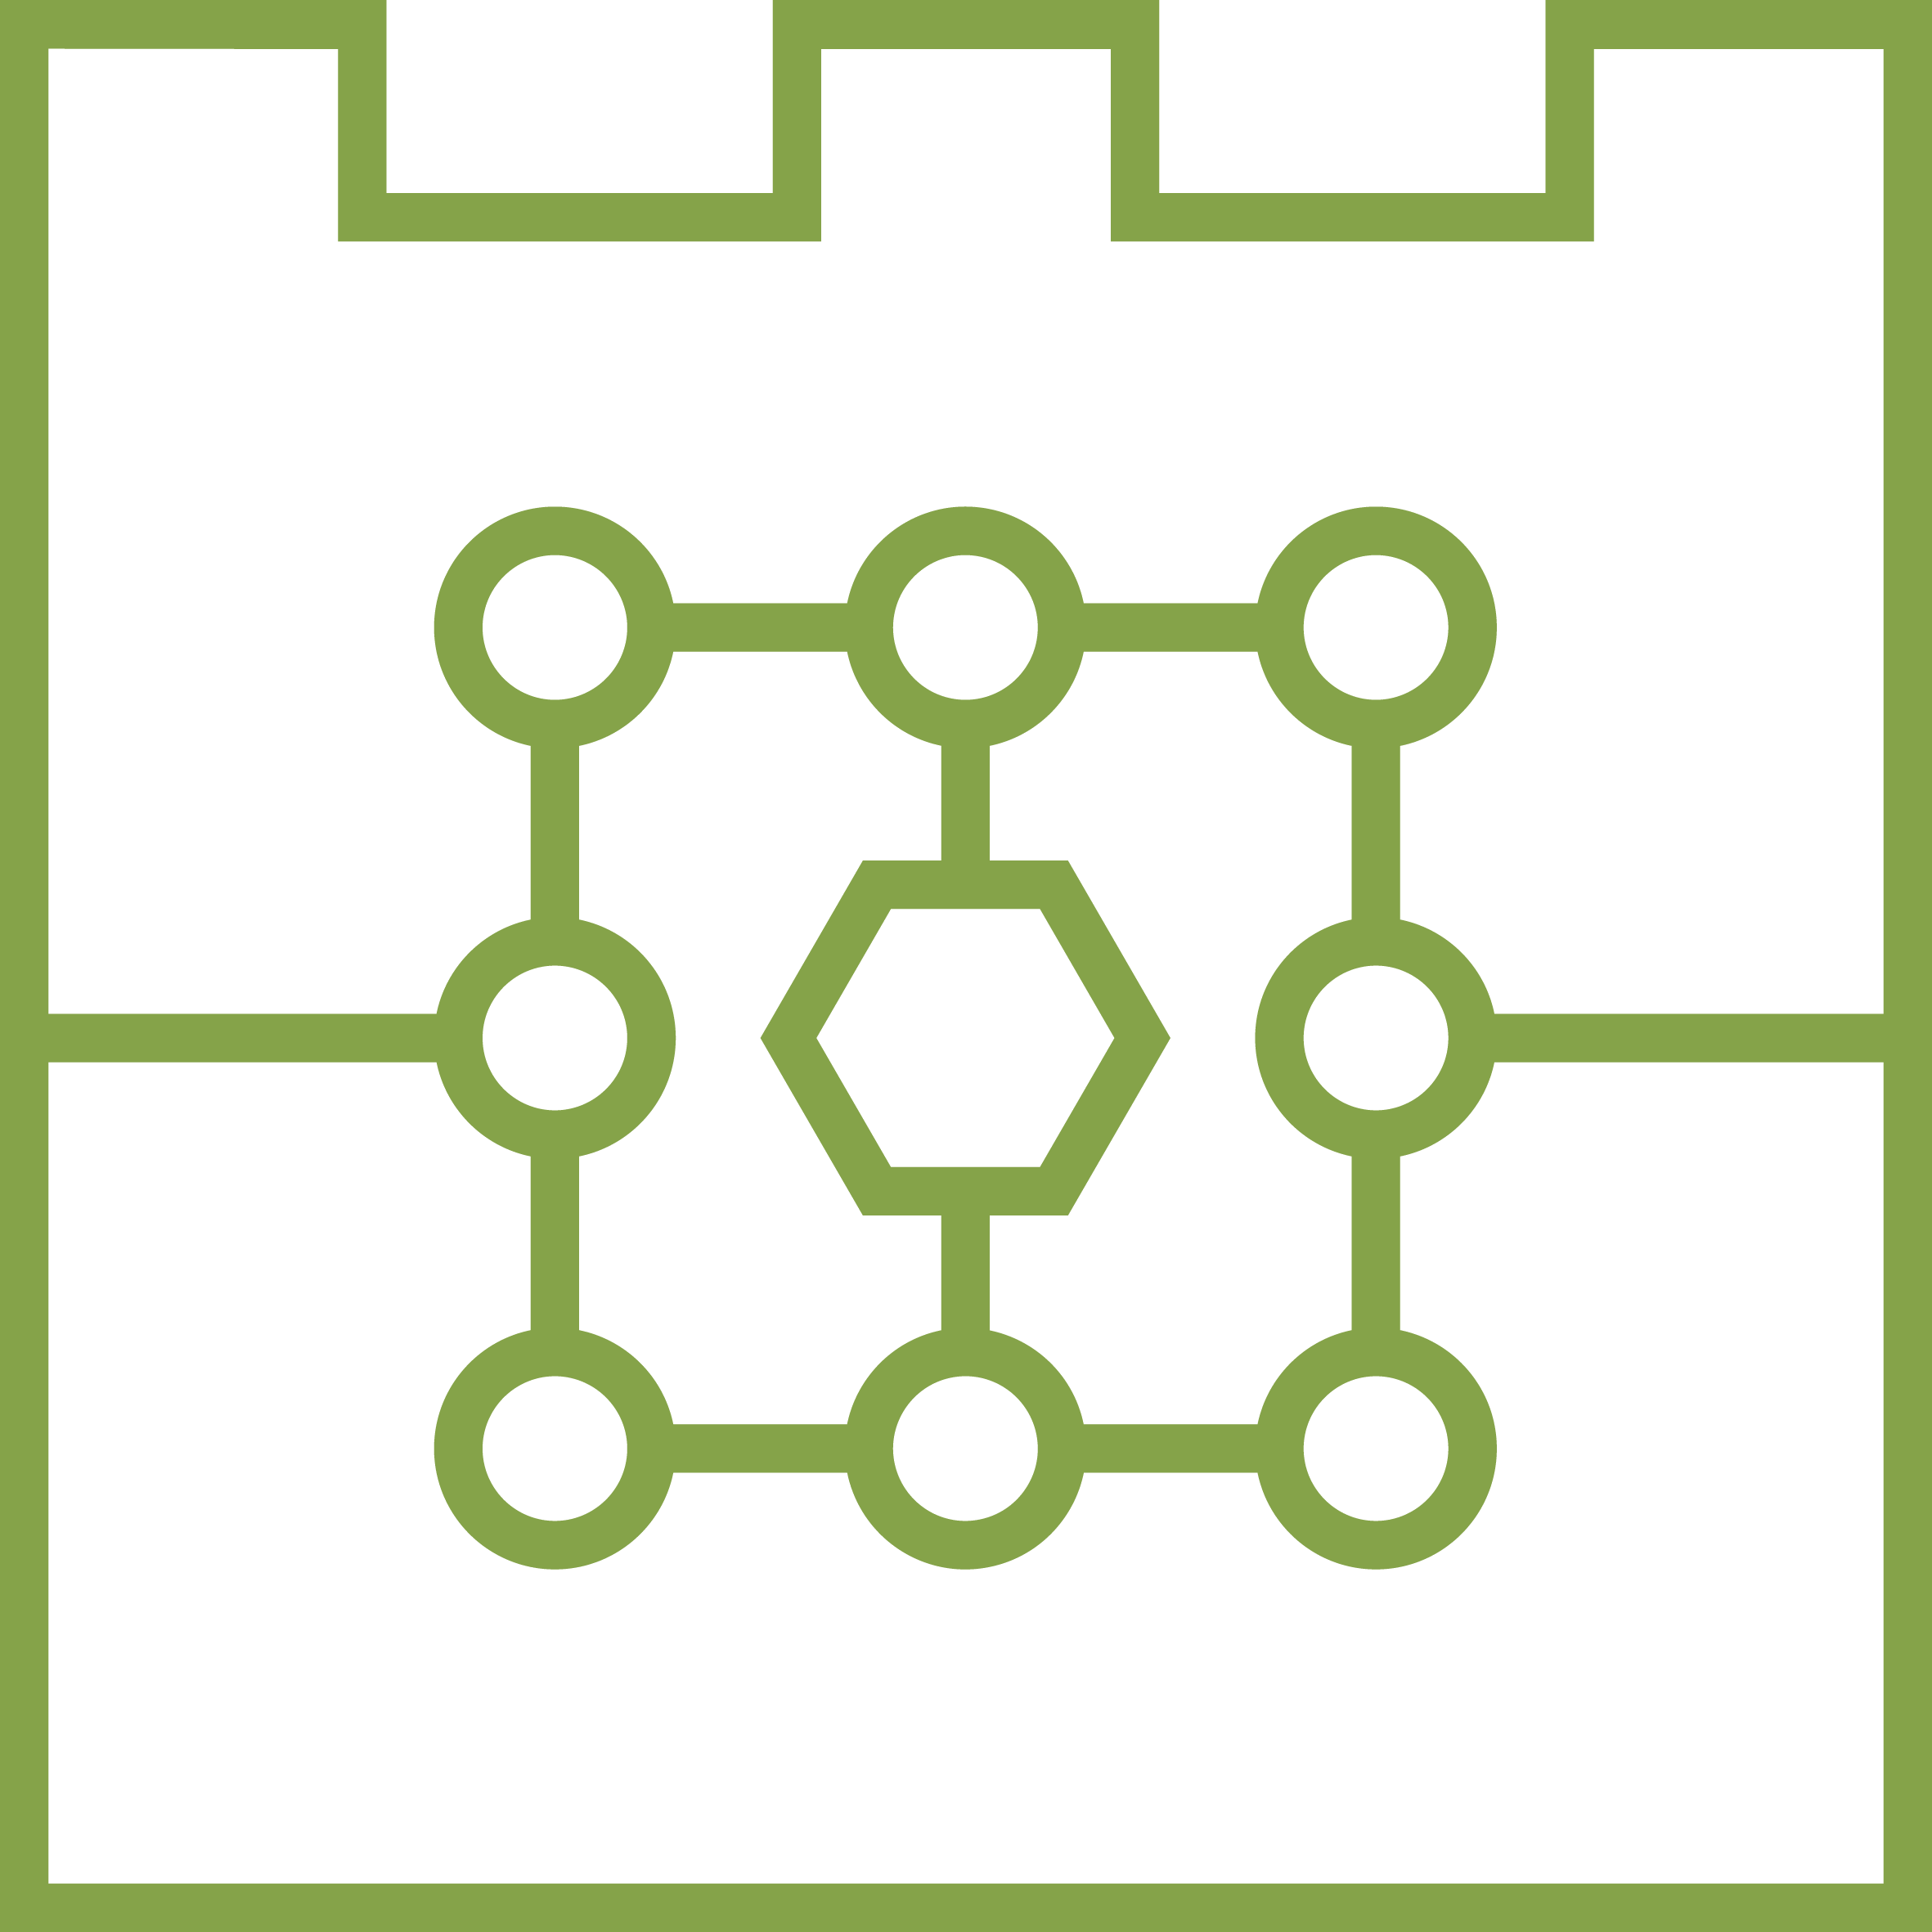
\includegraphics[width=0.15\textwidth]{logo_pk/logoIT.png}}%\hspace{0.12em}
\parbox[c]{0.15\textwidth}



 \vspace{0.10\textheight}

 \center{\autor}
 \smallskip
 \center{\large numer albumu: \album}

\vspace*{2ex}

 \center{\pltitle}

 \smallskip

 \center{\engtitle}

 \bigskip

 \center{\Large\bfseries Praca \level \\[0.2ex] %jeśli magisterka to trzeba sobie przystosować pamiętając o specjalności
\fontfamily{qhv}\fontshape{n}\selectfont\Large\bfseries na kierunku
 \kierunek\\[0.2ex]
 }

\vspace{0.11\textheight}

\hspace{0.57\textwidth} \parbox{0.42\textwidth}{Praca przygotowana pod
kierunkiem:
\\
%
\bfseries \promotor}

\vfill

 % wpisać rok
 \center{Kraków, \rok}
 \end{titlepage}

 \newpage

% \vspace*{17cm}
% \begin{flushright}
% \textit{Tu można sobie coś wpisać}
% \end{flushright}






\chapter*{Abstrakt}
Niniejsza praca bada zależności pomiędzy parametrami akustycznymi, tekstami i 
cechami utworów muzycznych przy użyciu metod sztucznej inteligencji. Opracowano
i przeanalizowano zbiór danych utworów, obejmujący metadane Spotify, cechy
akustyczne, teksty piosenek oraz ścieżki mp3, w celu zbadania wzorców
związanych z tożsamością gatunkową, sentymentem i innymi właściwościami
utworów. Badania uwzględniają również, jak te cechy zmieniają się w czasie.
Wykorzystując rozbudowaną inżynierię cech, dogłębną eksploracyjną analizę
danych, przetwarzanie języka naturalnego, techniki uczenia maszynowego,
modelowanie tematów oraz metody statystyczne, praca analizuje relacje między
elementami muzycznymi i tekstowymi. Opracowano i zinterpretowano modele
predykcyjne za pomocą metod wyjaśnialnej sztucznej inteligencji, co zapewnia
przejrzystość i dostarcza cennych wniosków na temat branży muzycznej.

\chapter*{Abstract}
This thesis explores the relationships between acoustic parameters, lyrics, and
the characteristics of music tracks using artificial intelligence methods. It
creates and analyzes a dataset of songs, including Spotify metadata, audio
features, lyrics, and mp3 tracks, to study patterns related to song popularity,
genre identity, sentiment, and other song characteristics. The research also
examines how these properties evolve over time. Using comprehensive feature
engineering, thorough exploratory data analysis, natural language processing,
machine learning techniques, topic modeling, and statistical methods, it
investigates connections between musical and lyrical elements. Predictive
models are developed and interpreted with explainable AI methods to ensure
transparency, providing valuable insights into the music industry.






\tableofcontents
\clearpage

\chapter{Introduction}
\label{cha:introduction}

\section{Problem Statement}
\label{sec:problemstatement}
Music has been a prominent part of human culture for generations. It's been
evolving alongside societies, reflecting their creativity, emotions, values and
emerging trends. In this day and age music has become more accessible and
popular than ever, especially thanks to advancements in technology. Rapidly
expanding global audience, growing number of artists and overwhelming number of
songs released every day presents us with a great opportunity to investigate
more closely its characteristics through the lens of data-driven analyses and
machine learning techniques. 

Based on the acoustic features that can be extracted from the music tracks, and
textual features extracted from song lyrics and information available on
Spotify, this study attempts to understand better complex relationships between
different music track characteristics and uncover insights into how music is
perceived by listeners, the factors that influence song's popularity, the
defining traits of various music genres and how trends shape the evolution of
music and its characteristics over the years. 

This approach offers a modern, quantitative perspective on music, enabling us
to further explore relationships between different musical and textual
characteristics.




% \begin{center}
% \begin{figure}[ht]
%   \centering
%   
\includegraphics[width=6in]{img/plik.png}
%   \caption{Podpis pod rysunkiem\cite{nature_behavior}.}
%   \label{Figure:fig_beh}
% \end{figure}
% \end{center}

%---------------------------------------------------------------------------

\section{Research Questions \& Objectives}
\label{sec:researchquestions}
% This thesis aims to leverage a diverse dataset of songs collected through a
% systematic metehodology, consisting of metadata, Spotify's audio features,
% lyrics and mp3 tracks. 

The aim of this thesis is to build a diverse dataset of songs with lyrical,
acoustic and metadata features through a well-defined data collection
methodology and use various advanced data analysis methods and explainable
artificial intelligence (\textit{XAI}) to:

\begin{enumerate}
  \item Explore the relationships between lyrical, acoustic, and metadata
    features of songs to uncover meaningful patterns and dependencies;
  \item Analyze defining characteristics of songs across different genres and
    investigate how these features contribute to genre identity and what are
    defining traits for each genre included in the dataset;
  \item Develop predictive models to estimate various song attributes (e.g.
    popularity, explicitness, sentiment) and use XAI methodologies to interpret
    model's predictions and extract meaningful insights and relationships;
  \item Identify commonly recurring themes in lyrics and explore their
    significance and distinctive traits using topic modelling;
  \item Uncover temporal trends and shifts in music characteristics over time.
\end{enumerate}

Additionally, this thesis aims to create a practical and reusable explainable
AI(\textit{XAI}) evaluation framework and a clear and systematic method for
collecting data. These tools are designed to make it easier to build on this
work, apply the methods to new projects and research.


%---------------------------------------------------------------------------


\section{Thesis Structure}
\label{sec:thesisstructure}

This thesis begins with an introduction and explaination of research objectives.
It's followed by a discussion of related studies, summarizing each of them and
explaining how  they relate to this work. 

The data chapter explains the sampling method that was used to select the songs
from Spotify, the data collection framework, the sources for the data and the
data itself.

Next, the methodology chapter outlines the feature engineering process,
describing all extracted features, and introduces all the techniques
and methods used in this study. 

The chapter that comes after that describes the extensive exploratory data
analysis conducted on the collected data with the aim of exploring relationships
between features and identifying distinctive traits of each genre.

The experiments chapter presents all the experiments conducted in this study
and discusses their results. It also compares them to different benchmarks and
attempts to interpret the results.

The thesis concludes with a summary of contributions, a description
of the limitations, key findings, and recommendations for future work. 

\chapter{Related Work}
\label{cha:literaturereview}

%---------------------------------------------------------------------------

\section{Acoustic Features in Music Analysis}
\label{sec:acousticfeaturesinmusicanalysis}

\subsubsection*{``Music Genre Classification Using MFCC, k-NN, and SVM
Classifier``}


This study explores music genre classification using MFCCs and Chroma features
on the GTZAN dataset, that consists of 900 tracks across 9 genres. The
best-performing model was an SVM with a polynomial kernel, achieving accuracy
of 78\%. Some genres were identified to have overlapping characteristics which
posed problems for the classification model.\cite{music_genre_classification_mfcc}

The paper highlights the effectiveness of MFCCs and Chroma features for
audio-based classification, aligning with this thesis's use of acoustic
features. However, unlike this study, the thesis extends the analysis by
incorporating lyrical features, metadata, and audio features provided by
Spotify, addressing limitations in feature diversity.

\subsubsection*{``Classifying Music Audio with Timbral and Chroma Features``}

The paper ``Classifying Music Audio with Timbral and Chroma Features`` examines
the use of timbral (e.g., MFCCs) and harmonic (e.g., chroma) features in music
classification tasks. The study highlights that MFCCs, which represent timbral
qualities, are effective for tasks like \textbf{artist identification, achieving 56\%
accuracy in a 20-way classification task}. When combined with beat-synchronous
chroma features, which capture harmonic and melodic information, the model's
accuracy improved to 59\%. This demonstrates the importance of leveraging
complementary audio features for more robust classification. These findings
emphasize the potential of combining diverse acoustic features in predictive
models, aligning closely with the objectives of this thesis.\cite{classifying_music_audio}



%---------------------------------------------------------------------------

\section{Lyrical Features in Music Analysis}
\label{sec:lyricalfeaturesinmusicanalysis}

\subsubsection*{``Using Machine Learning Analysis to Interpret the Relationship
Between Music Emotion and Lyric Features``}


This study investigates the relationship between lyrical features and perceived
music emotions using 2,372 Chinese pop songs. Lyric features were extracted
with LIWC (Linguistic Inquiry and Word Count), and audio features
such as MFCCs and chroma were derived using Librosa. The analysis highlighted
that lyrical features like the frequency of positive and negative emotion words
contributed significantly to predicting the perceived valence of music, whereas
audio features were dominant in predicting perceived arousal.\cite{valence_and_lyrics}

The study utilized Random Forest regression models, demonstrating that
combining lyric and audio features improved \textbf{predictions of valence,
with an $R^2$ of 0.481}, but lyrics had little impact on arousal models. These
findings align with this thesis's use of both lyrical and acoustic features for
predictive tasks but differ in the application of explainable AI (XAI)
techniques like SHAP for feature interpretation. Moreover, this thesis expands
this study by incorporating Spotify audio features and metadata for broader
analytical capabilities and more diverse research objectives.


\subsubsection*{``Sentiment Analysis and Lyrics Theme Recognition Using NLP Techniques``}


This paper investigates the relationship between sentiment and themes in music
lyrics using Natural Language Processing (NLP) techniques. It applies sentiment
analysis and thematic recognition across a diverse dataset, identifying
emotional nuances and recurring topics in the lyrics. The analysis identifies
correlations between sentiment categories (positive, negative, neutral) and
thematic clusters (e.g., love, social justice, personal reflection). The
authors use techniques like Latent Dirichlet Allocation (LDA) for topic
modeling and Support Vector Machines (SVM) for sentiment classification.\cite{du_2024}

In the context of this thesis, this study aligns closely with the focus on
lyrical analysis, particularly in employing NLP-driven sentiment and thematic
classification. However, while this work emphasizes standalone lyric-based
analysis, this thesis extends the methodology by integrating Spotify’s audio
features, acoustic analysis, and metadata. 

%---------------------------------------------------------------------------

\section{Machine Learning in Music Analysis}
\label{sec:machinelearningfeaturesinmusicanalysis}

\subsubsection*{``Beyond Beats: A Recipe to Song Popularity? A Machine Learning Approach``}

The paper ``Beyond Beats`` investigates the predictive power of various machine
learning models for song popularity on a dataset of 30,000 songs spanning six
genres. It focuses on metadata and audio features fetched from
Spotify (\textit{danceability}, \textit{acousticness} etc.), as well as the
genre. The best performing model was \textbf{Random Forest and achieved 16.31 MAE.}
Predictions across all methods remained relatively modest, reflecting the
complex and multi-dimensional  nature of song popularity. Those results can be
greatly improved using additional features. The authors noted that predictive
accuracy was constrained by the absence of post-release factors such as
marketing, social media reception, and artist reputation.\cite{beyond_beats}


\subsubsection*{``Predicting Song Popularity in the Digital Age Through
Spotify’s Data``}  
Similarily to the previous one, the paper ``Predicting Song Popularity in the
Digital Age Through Spotify’s Data`` explores the relationship between
Spotify's audio features  and song popularity, using a dataset spanning from
1986 to 2022. The study employed linear regression to predict popularity and
\textbf{achieved an adjusted $R^2$ of 0.38}, highlighting the moderate
predictive power of these features. The analysis revealed that attributes such
as \textit{danceability} and \textit{duration} positively correlate with
popularity, while \textit{speechiness} tends to have a negative
impact.\cite{predicting_song_popularity_2024}

\chapter{Data}
\label{cha:data}


%---------------------------------------------------------------------------

\section{Sampling Method}
\label{sec:samplingmethod}


Spotify’s catalog contains approximately 100 million songs and over 6000
distinct genres. Collecting a truly random sample from this huge and diverse
population presents significant challenges. A purely random sampling approach
would likely result in a dataset heavily skewed towards obscure genres and
imbalanced release year distribution. This would lead to poor data quality for
meeting the research objectives, with sparse meaningful relationships and an
overwhelming diversity of genres. Such diversity would make it nearly
impossible to extract actionable insights and relationships, as less
represented genres and rare tracks would dominate, shifting the focus from more
prominent trends and patterns in music.


To address these challenges, a smaller and more organized sample of 3500 songs
was selected. The stratified sampling approach was designed to ensure a
balanced dataset by focusing on two key factors: genre and release year. The
sampling process utilized Spotify's query parametrization tool, which allows
for the specification of desired genres and release year ranges for musical
tracks. Release years were grouped into 10-year intervals, starting from 1950
and extending to 2020, ensuring the dataset represents different time periods
in modern music. The selection of genres was arbitrary and aimed to include a
mix of popular and diverse styles, providing a robust representation of
mainstream musical styles.

Additionally, in order to enable more precise and insightful topics extraction
and uniformity of the data, all songs whose lyrics weren't identified to be in
English were discarded.
 
While this approach introduces some degree of selection bias, favoring tracks
that Spotify's search algorithm prioritizes, this bias is acceptable given the
research objectives. By explicitly focusing on popular genres and balancing
across release years, the sample aims to capture relationships and patterns
that are representative of mainstream trends and music evolution. The
structured stratification ensures that each genre and time period is adequately
represented, providing a comprehensive and interpretable dataset for  the
analysis.


%---------------------------------------------------------------------------

\section{Dataset Description}
\label{sec:datasetdescription}

The dataset consists of around 3500 songs in English. For each song metadata, audio
recording, lyrics and spotify audio features were fetched.

\section{Data Collection Methods}
\label{sec:datacollectionmethods}

\subsection{Sources}
The data was collected from various sources. Metadata and audio features were
fetched from Spotify API. The lyrics were scraped from LetrasMus,
MakeItPersonal or Lyrics Fandom, or fetched via the Genius API, depending on
the availability. Audio files were downloaded from YouTube using youtube-dl
library and saved as mp3 files.\cite{spotify_api} \cite{makeitpersonal}
\cite{genius} \cite{letras_mus} \cite{lyricsfandom} \cite{ytdl} 

\subsection{Methodology}
The data collection process was automated for efficiency. The starting point
was a list of genres and decades. The script leveraged Spotify API's search
query parametrization to fetch equal number of songs from each genre and in
released in  each decade. For every song its metadata and audio featurers were
fetched.

Lyrics were then searched based on \textit{artist name} and \textit{title} of
each song, using multiple lyrics providers. The system continued to query
different sources until it found lyrics in at least one of them. If it failed
to retrieve lyrics for the song, it was discarded and wouldn't make it to the
final dataset.

Finally, the script  searched YouTube for each song and downloaded the first
relevant result, saving it to an mp3 file. All data was saved into a CSV
file named after the playlist and stored alongside the recordings.

The entire process was parallelized to significantly enhance the speed of data
acquisition. It was designed in a robust manner, with careful error handling
and ability to stop the process at any  time and pick up where it left off.


%---------------------------------------------------------------------------


\subsection{Metadata}
\label{sec:metadata}
Metadata included song's information downloaded from Spotify API, precisely:

\begin{itemize}
  \item \textbf{Popularity} - relative measure with values ranging from 0 to
    100 describing how popular the song is, estimated mostly based on total
    number of plays and how recent  those plays are.
  \item \textbf{Explicitness} - whether or not the song contains explicit
    lyrics.
  \item \textbf{Genre} - the genre specified in the search query that returned
    this song.
  \item \textbf{Album Release Year} - the release year of the album that the
    song originates from.
\end{itemize}


\subsection{Spotify Audio Features}
\label{sec:spotifyaudiofeatures}
Those features were fetched from the Spotify API.They describe different
acoustic properties of the songs:
\begin{itemize}
  \item \textbf{Speechiness} - relative measure of spoken words in a track.
  \item \textbf{Acousticness} - a confidence measure of whether the song is
    acoustic.
  \item \textbf{Danceability} - a measure of how suitable the song is for
    dancing. Its based on parameters like tempo, rhythm stability, beat
    strength etc.
  \item \textbf{Energy} - a measure of perceived intensity of songs. Energetic
    tracks are usually louder, faster, feel more intense.
  \item \textbf{Loudness} - overall loudness of the  track in dB averaged
    across the entire track.
  \item \textbf{Valence} - relative measure describing musical positiveness of
    a track.
  \item \textbf{Instrumentalness} - likelihood of the track not containing
    vocals. In this paper since lyrics are mandatory it's used to discard
    instrumental tracks.
  \item \textbf{Liveness} - probability of the song being recorded during a
    live performance.
  \item \textbf{Key} - the key of the song, e.g. C\#.
  \item \textbf{Mode} - indicates the modality of a track(major / minor).
  \item \textbf{Tempo} - estimated tempo of a track in beats per minute(BPM).
  \item \textbf{Time Signature} - specifies how many beats there are in each
    bar.
  \item \textbf{Duration} - the duration of the track in milliseconds.
\end{itemize}


\subsection{Lyrics Features}
 The lyrics serve as a textual representation of the song's thematic,
 emotional, and linguistic elements. Since they came from various data sources,
 they had  to undergo cleaning procedure in order to remove faulty information
 and prepare them to be processed by the text features extraction class. The
 process consisted of:
 \begin{itemize}
  \item \textbf{Standardization} - lyrics were converted to lowercase.
  \item \textbf{Noise Removal} - unnecessary characters, numbers and
    punctuation, as well as additional comments used by lyrics providers(e.g.
    'chorus') were removed.
  \item \textbf{Stopwords Filtration} - exclusion of frequently occuring words
    that carry little information, like 'the' in English.
  \item \textbf{Stemming} - words were reduced to their root forms to enhance
    uniformity and reduce corpus size.
 \end{itemize}

 This process laid foundation for further extraction of textual features used
 for exploratory data analysis, statistical inference and training ML models.
 That process will be explained in later chapter.


%---------------------------------------------------------------------------

\section{Tools and Libraries Used}
\label{sec:toolsandlibrariesused}
Python libraries used to for data acquisition were:
\begin{itemize}
  \item \textit{Spotipy} - a lightweight python library for
    Spotify API.
  \item \textit{youtube-dl}  - a library used to find and download
    YouTube videos.
  \item \textit{BeautifulSoup}  - a library used for
    extracting information from HTML, commonly used for web scraping.
\end{itemize}

References: \cite{spotipy} \cite{ytdl} \cite{beautifulsoup}


\chapter{Methodologies}
\label{cha:methodologies}



Throughout this chapter, the methodologies used to approach the research
objectives are explained. It describes the feature engineering and extraction
methods, the way explainable AI methods are used, model training and
optimization approaches, clustering and dimensionality reduction techniques and
statistical hypotheses testing methods.
%---------------------------------------------------------------------------

\section{Feature Engineering}
\label{sec:featureengineering}

Feature engineering is a vital step in the research process, as it involves
transforming raw data acquired using the data collection script into meaningful
representations that can be analyzed or used for predictive modeling. In this
section the methodologies used to get acoustic features from the mp3 files and
lyrical features from the lyrics are described. These features are designed to
capture key characteristics of the songs, enabling deeper insights into their
patterns and relationships.


\subsection{Acoustic Features}
\label{sec:acousticfeatures}

These features provide a numeric representation of the acoustic properties of
each song and were extracted directly from the audio files in MP3 format. They
describe different aspects of audio signal and provide information about the
rhythm, timbre, harmony and other acoustic properties. The extraction was done
using \textit{Librosa} and was automated and parallelized to make it suitable
for processing large amounts of data. \cite{librosa}


\subsubsection*{MFCC - Mel Frequency Cepstral Coefficients}
MFCCs are used to analyze the short-term power spectrum of a song on a
mel-scale. They're also used for timbre analysis, and they capture the tonal
quality of the audio, which helps differentiate between different instruments
and vocal characteristics.


\subsubsection*{Chroma}
Chroma vectors represent the intensity of each pitch class (e.g., C, C#, D, etc.) in the audio.
These features provide a harmonic representation of the song and are useful for analyzing
chord progressions and harmonic structures.

\subsubsection*{Spectral Contrast}
Spectral contrast measures the difference in amplitude between peaks and
valleys in the spectrum. It provides insights into the harmonic and timbral
content of a song, particularly useful for distinguishing between smooth and
complex textures.

\subsubsection*{Other Features}
Two additional features were extracted:
\begin{itemize}
  \item \textbf{Tempo} - speed of the song, measured in
    \textit{Beats Per Minute(BPM)};
  \item \textbf{Zero Crossing Rate(ZCR)} - measures the rate at which the audio
    signal changes sign. Commonly used as a measure of noisiness or
    percussive nature of signal.
\end{itemize}

%---------------------------------------------------------------------------

\subsection{Lyrical Features}
\label{sec:lyricalfeatures}

Lyrical features  were extracted from the lyrics fetched during the data
collection process. They aim to provide a linguistic and semantic
representation of the track, capturing their complexity, sentiment and
stylistic  attributes. In the cleaning and extraction  process various NLP
libraries like \textit{NLTK}, \textit{spaCy} and \textit{TextBlob} were used,
alongside with custom ad-hoc algorithms. Before extraction the lyrics  had to
be carefully cleaned, removing unnecessary characters and stopwords, performing
stemming etc.\cite{nltk} \cite{spacy} \cite{textblob} 

Similarily to acoustic features the implementation allowed for simple and
intuitive usage  with parallelization of the computation process for increased
performance. 

The features extracted can be grouped as follows:

\subsubsection*{Basic Linguistic Metrics}
\begin{itemize}
  \item \textbf{Unique Word Count} - measures number of unique words in the
    lyrics, indicating diversity;
  \item \textbf{Type-Token Ratio} - measures of lexical richness: ratio of
    unique words to total words;
  \item \textbf{Word Count} - total  number of words;
  \item \textbf{Noun and Verb Ratios} - proportions of nous and verbs relative
    to the total word count.
\end{itemize}


\subsubsection*{Sentiment and Emotional Tone}
\begin{itemize}
  \item \textbf{Sentiment Polarity} - a measure of overall sentiment(positive
    vs. negative) of the text;
  \item \textbf{Sentiment Subjectivity} - represents the degree of subjectivity
    in the lyrics;
  \item \textbf{VADER Compound} - a sentiment score obtained using VADER;
  \item \textbf{Sentiment Variability} - standard deviation of sentiment on
    subsets of lyrics. This metric aims to capture changes in sentiment
    throughout the song.
\end{itemize}


\subsubsection*{Stylistic Features}
\begin{itemize}
  \item \textbf{Repetition Count} - the frequency of repeated words;
  \item \textbf{Rhyme Density} - a measure of how often rhymes occur in the
    text;
  \item \textbf{Linguistic Uniqueness} - ratio of rarely used words to all the
    words in the song.
\end{itemize}


\subsubsection*{Semantic and Complexity Features}
\begin{itemize}
  \item \textbf{Semantic Depth} - represents the richness and variety of
    meaning of the lyrics;
  \item \textbf{Syntactic Complexity} - captures the sophistication of
    sentence structures;
  \item \textbf{Lexical Richness} - quantifies the variety and richness of the
    vocabulary.
\end{itemize}



\subsubsection*{Readability and Accessibility}
\begin{itemize}
  \item \textbf{Flesch Reading Ease} - indicates how easy the lyrics are to
    read;
  \item \textbf{Gunning Fog} - a metric that estimates the  years of education
    required to understand the text;
  \item \textbf{Dale Chall} - a metric that accounts for familiar and
    unfamiliar words in the text.
\end{itemize}


\subsubsection*{Contextual Information}
  In process of feature extraction the \textbf{language} of lyrics was also
  identified using \textit{langdetect} library. Langdetect uses a
  classification model to predict the language of a text based on n-grams from
  it. The identified language was also used cleaning process, to remove songs
  that weren't in English.

\subsubsection*{TF-IDF (Term Frequency - Inverse Document Frequency)}

TF-IDF is a measure that can quantifies the relevance of tokens in a
document in a collection of documents. It's used to highlight words that are unique or
meaningful while giving less importance to very common words like 'the' or
'and'.\cite{tfidf}

It can be broken down into two parts:


\begin{itemize}
  \item \textbf{TF - Term Frequency} - Measures the frequency of a term within
    a document:
  \[
  TF(w, d) = \frac{f_{w, d}}{N_d}
  \]
  where:
  \begin{itemize}
    \item \( f_{w, d} \): The number of times the word \( w \) appears in the
      document \( d \);
    \item \( N_d \): The total number of words in the document \( d \).
  \end{itemize}

  \item \textbf{IDF - Inverse Document Frequency} - Measures the rarity of a
    term across a collection of documents:
  \[
  IDF(w) = \log{\frac{N}{1 + n_w}}
  \]
  where:
  \begin{itemize}
    \item \( N \): The total number of documents in the corpus;
    \item \( n_w \): The number of documents containing the word \( w \).
  \end{itemize}
\end{itemize}


The final TF-IDF value is calculated by multiplying the Term Frequency (TF) and
the Inverse Document Frequency (IDF) for a word \( w \):  
\[  
TF\text{-}IDF(w, d) = TF(w, d) \cdot IDF(w)  
\]  

Terms that occur frequently in a specific document(high TF) and rarely appear
in other documents (high IDF) receive a higher score.

\subsubsection*{Word2Vec}

Word2Vec is a neural network-based technique in NLP for creating dense vector
representations of words. These vectors capture information about the meaning
of words based on the surrounding words. Unlike bag-of-words or TF-IDF methods,
Word2Vec generates embeddings that preserve the contextual meaning of words
based on their usage within the corpus.\cite{w2v}

Two primary approaches are used in Word2Vec: 
\begin{itemize} 
  \item \textbf{Continuous Bag of Words}: Predicts a target word based
    on its surrounding context words;
  \item \textbf{Skip-Gram}: Predicts context words given a target word.
\end{itemize}

In this study, Word2Vec was used to create vector representations of song
lyrics. These embeddings  were used similarily to TF-IDF, as input features
to predictive models and when comparing lyrical similarities between genres.



\subsubsection*{Empath}
Empath is a semantic analysis tool designed for extracting
semantic, thematic and emotional features from text by analyzing words based on
predefined categories. It classifies words into over 200 built-in categories,
such as \textit{sadness}, \textit{food} and \textit{music}. It  identifies
relationships between words and these categories, offering a higher-level
representation of text content beyond simple word frequency.\cite{empath}

In this study Empath was used to analyze song lyrics by extraction of 
interpretable features describing song's thematic and emotional content.
Those features were used in the predictive models developed for various
tasks and in exploratory data analysis. Empath's clearly defined  categories 
enhanced the interpretability of genres and topics identified by LDA, 
making it easier to understand distinctive traits of songs that belonged to
them.

By combining Empath with traditional feature extraction methods, this study
benefits from a richer, more interpretable representation of lyrical content.

%---------------------------------------------------------------------------

\section{Explainable AI Methods}
\label{sec:explainableaimethods}

Explainable AI (XAI) are becoming more and more popular as the complexity of
models and amounts of data grow, increasing the need to investigate model's
decision-making processes and better understand the impact that features have
on the model's predictions. XAI techniques enable model  transparency and can
be used as a  tool to better understand the relationships in the training data,
by exploring the impact the features have on the target variable. 

In this study this methodology was applied in various experiments to understand
how specific variables influence others, providing insight into the most
important features and their interactions with the target variable in each
prediction task specified in the research objectives.



\subsubsection*{SHAP (SHapley Additive exPlanations)}

SHAP (SHapley Additive exPlanations) is a framework used to interpret
predictions made by various predictive models based on game-theoretic approach.
SHAP values attribute to each feature the change in the expected model
prediction when conditioning on that feature, providing a unified measure
of feature importance.\cite{shap}

In this study SHAP values were used to explain the predictive process
of trained Catboost models, by exploring the feature importance and
visualization of relationships between the features and target variable.

\begin{center}
  \begin{figure}[H]
  \centering
  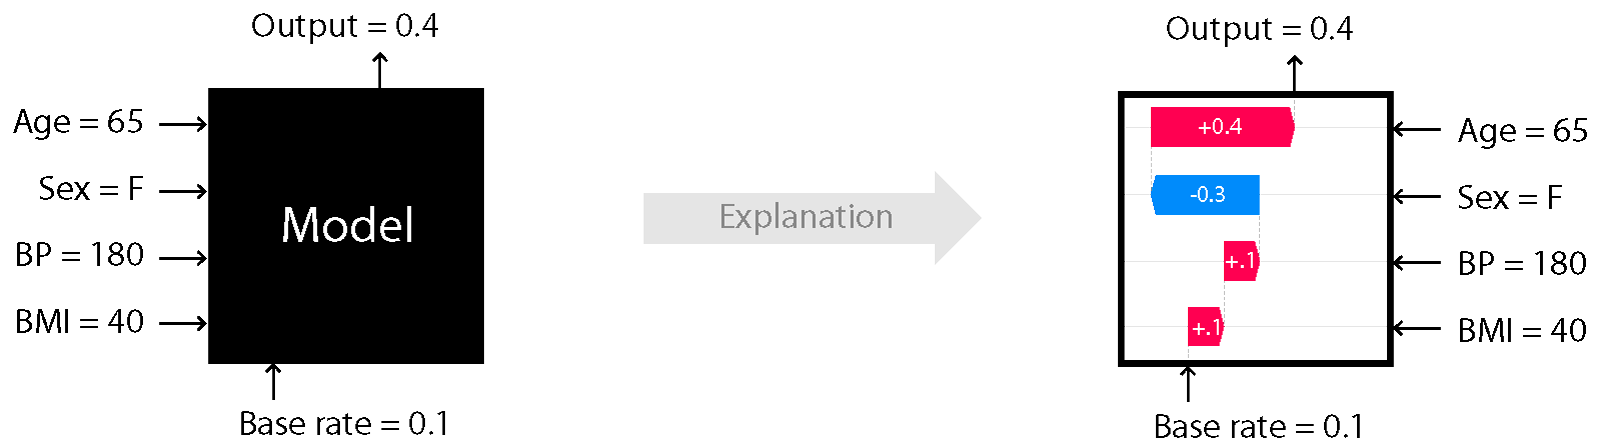
\includegraphics[width=4in]{img/shap_intro.png}
  \caption{SHAP}
  \label{Figure:fig_beh}
\end{figure}
\end{center}

\begin{center}
  \begin{figure}[H]
  \centering
  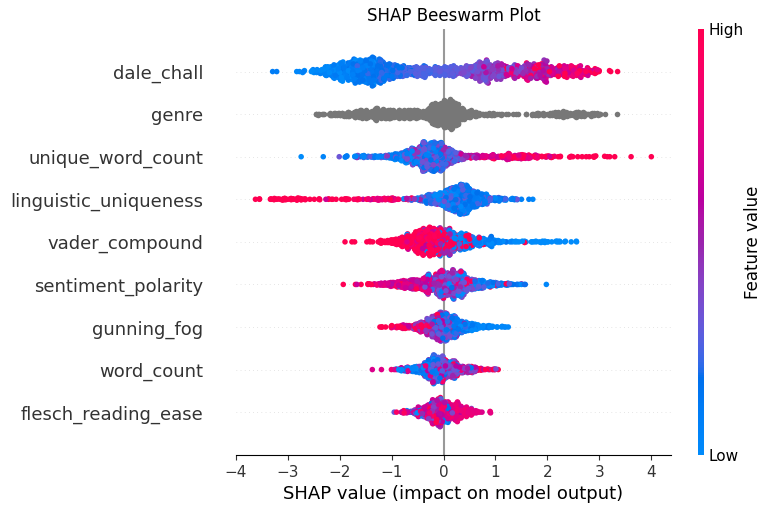
\includegraphics[width=4.5in]{img/shap_beeswarm.png}
  \caption{Example SHAP beeswarm plot showing impact of some lyrical features
  on the classifier of \textit{explicitness}.}
  \label{Figure:fig_beh}
\end{figure}
\end{center}

\begin{center}
\begin{figure}[H]
  \centering
  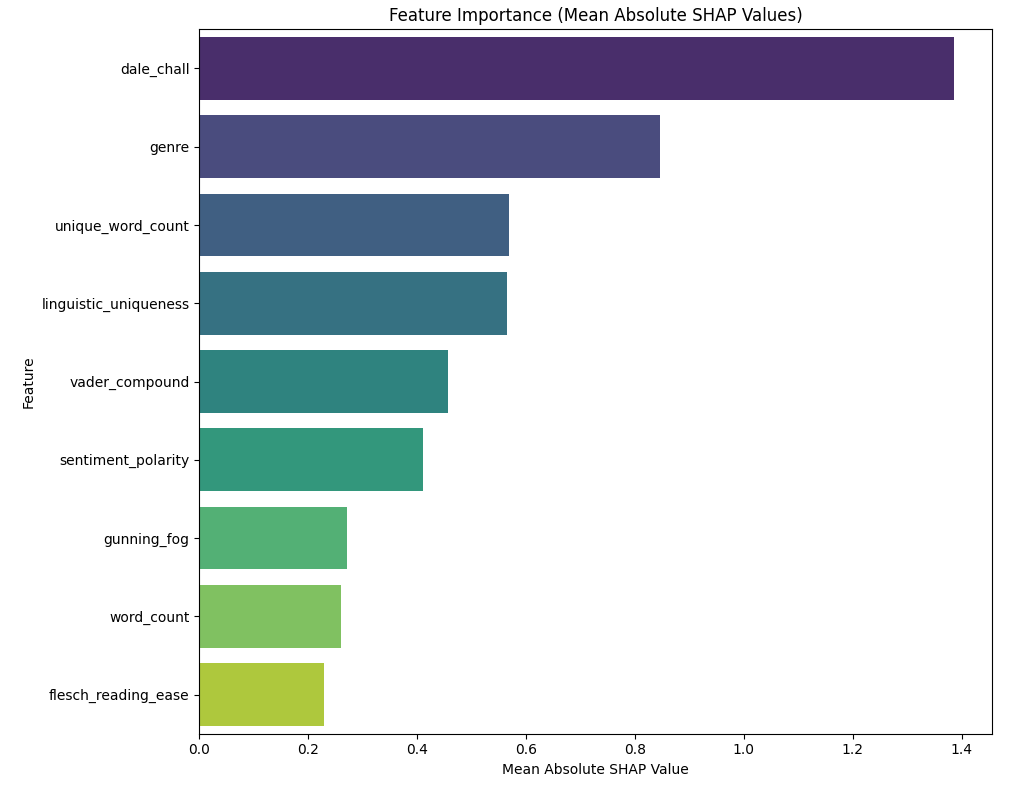
\includegraphics[width=3in]{img/shap_feature_importance.png}
  \caption{Example SHAP feature importance plot showing impact of some lyrical features
  on the classifier of \textit{explicitness}.}
  \label{Figure:fig_beh}
\end{figure}
\end{center}
%---------------------------------------------------------------------------

\subsubsection*{Machine Learning Models}
CatBoost is an algorithm for gradient boosting on decision trees. It's known
for its high predictive accuracy, even without extensive parameter tuning, and
its computational efficiency. In this study it was used to build several
classification and regression models, with the goal of variables like
popularity or explicitness on different subsets of features from the dataset.
The trained models were then subjected to SHAP analysis, uncovering their
decision processes and helping to understand the interactions between the
features and the target variable. Catboost's flexibility, robustness,
compatibility with SHAP and ability to automatically handle categorical
variables and class imbalance.\cite{catboost}


In order to further optimize the performance of the models, the
hyperparameter tuning library \textit{Optuna} was used. Optuna is an
efficient optimization framework that allows to systematically test different
sets of hyperparameter configurations, ensuring the final model achieves
optimal performance.\cite{optuna} 

To address the challenges commonly encountered when training ML models on
complex datasets, following techniques were employed:

\begin{itemize}
  \item \textbf{Cross-validation} - cross-validation was used to reduce the
    risk of overfitting and provide a way to reliably calculate model's
    performance metrics. In principle it consists of dividing the training
    data into multiple \textit{folds}, and the model is iteratively trained
    on all folds but one, and evaluated on the one that didn't participate in
    training. In each iteration a different fold is chosen as the evaluation
    fold. This method ensures robust evaluation across the dataset and improved
    model's reliability, at the cost of increased computational time;
  \item \textbf{Class Weights} - due to natural imbalances or skweness in the
    data that was collected, in most classification tasks discussed in this
    paper the target variable(e.g. explicitness) had different number of samples
    representing each value(e.g. there were many more non-explicit songs). That
    kind of imbalance would lead to model favouring the majority class, and
    therefore performing poorly. Catboost offers a built-in mechanism to handle
    class imbalance by assigning different penalties for misclassifications
    of specific classes, improving model's performance across all classes;
  \item \textbf{Out of sample evaluation} - model's performance was evaluated
    on data that was completely excluded from the training process, ensuring
    reliable measurement of model's ability to generalize on unseen data.
\end{itemize}

\section{Dimensionality Reduction - Principal Component Analysis (PCA)}
\label{sec:dimensionalityreduction}
Principal Component Analysis (PCA) is a dimensionality reduction technique
that reduces the number of features by transforming them into \textit{principal
components} that retain most of the original information. It works by
converting potentially correlated variables in to smaller sets of less correlated
variables, in a way that preserves as much of the variance from the original
data as possible. It's often applied on large datasets to reduce dimensionality
and improve generalization and performance by reducing noise and redundancy
in the data.\cite{pca}

In this study it was applied to the TF-IDF and Word2Vec vectors extracted from
the song lyrics. The vectors in their original form were problematic due  to
increased computational complexity and risk of overfitting the trained models.

The application of PCA reduced their dimensionality while preserving as much
useful information as possible, improving the computational efficiency and 
the interpretability of the data, which is particularly important in context of
XAI.

\begin{center}
\begin{figure}[H]
  \centering
  \includegraphics[width=4in]{img/pca.png}
  \caption{A scatterplot showing the relationship between PC1 and PC2 when PCA
  is applied to a dataset. PC1 and PC2 axis are perpendicular to each other.\cite{pca}}
  \label{Figure:fig_beh}
\end{figure}
\end{center}


\section{Topic Modelling - Latent Dirichlet Allocation (LDA)}
\label{sec:topicmodelling}

Latent Dirichlet allocation is an unsupervised machine learning algorithm used
for topic modeling to uncovering the central topics and their distributions
across the dataset.\cite{lda}

In this study LDA was applied on the lyrics to identify commonly occuring
topics in songs. The algorithm found optimal number of topics and they were
visualized using \textit{pyldavis}\cite{pylda} library. For each topic its most
representative words were extracted that in combination with other features
allowed to better characterize them and understand frequently occuring themes
in the lyrics.



\section{Statistical Methods}
\label{sec:statisticalmethods}

Statistical methods provided a foundation for descriptive data analysis, mainly
exploration of relationships between variables and identification of distinctive
genre traits, as well as hypothesis validation.

\subsection{Pearson Correlation}

It measures linear relationship between two continuous variables. The resulting
coefficient is a value between -1 to 1 and is computed as follows: 

\[
r = \frac{\sum{(x_i - \bar{x})(y_i - \bar{y})}}{\sqrt{\sum{(x_i - \bar{x})^2} \sum{(y_i - \bar{y})^2}}}
\]

\noindent \noindent Where:
\begin{itemize}
    \item \( x_i \) and \( y_i \): The data points of the two variables;
    \item \( \bar{x} \) and \( \bar{y} \): The mean values of the variables.
\end{itemize}

\noindent \noindent Interpretation:
\begin{itemize}
  \item An \textit{r} value close to 1 indicates very strong positive linear
    relationship;
  \item An \textit{r} value close to -1 suggests very strong negative linear
    relationship;
  \item An \textit{r} value close to 0 means there is little to no relationship.
\end{itemize}



\subsection{Bootstrap Testing}

Bootstrap testing was used to verify hypotheses specified in the research
objectives. It's a resampling-based statistical technique that estimates the
variability of a statistic(e.g. mean or median)  by repeatedly sampling its
values from the dataset with replacement. It's highly versatile since it
doesn't rely on strong distributional assumptions.


\begin{center}
\begin{figure}[H]
  \centering
  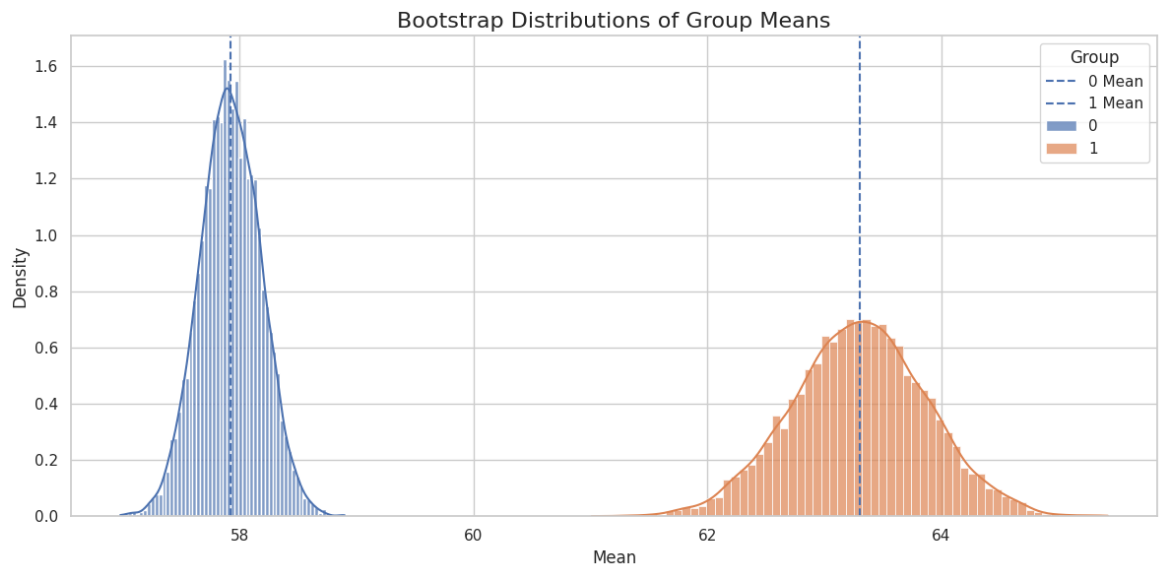
\includegraphics[width=5in]{img/bootstrap.jpg}
  \caption{Illustration of bootstrap resampling: The distribution of the
  statistic (e.g., mean) of the target variable for two different samples
(called groups). This demonstrates the variability of the statistic across
resampled datasets.}
  \label{Figure:fig_beh}
\end{figure}
\end{center}

\subsection{Analysis of Variance - ANOVA}
ANOVA is a statistical method used to compare the means of three or more groups
to determine if there is a statistically significant difference between them.
It tests the hypothesis that the means of all groups are equal against the
alternative hypothesis that at least one group mean is different.

\subsubsection*{Hypotheses}
\begin{itemize}
  \item \textbf{Null Hypothesis($H_0$)}: All group means are equal;
  \item \textbf{Alternative Hypothesis($H_a$)}: At least one group mean is
    different.
\end{itemize}

\noindent \noindent To verify the hypotheses two types of variation have to
be calculated:

\subsubsection*{Between-Group Variation}

This variation measures the differences between the means of groups. It
captures how much the group means differ from the overall mean.
\[
\text{Between-group \  variation} = \sum_{i=1}^{k} n_i (\bar{x}_i - \bar{x})^2
\]

\noindent \noindent Where:
\begin{itemize}
    \item \(n_i\): Number of samples in group \(i\);
    \item \(\bar{x}_i\): Mean of group \(i\);
    \item \(\bar{x}\): Overall mean.
\end{itemize}


\subsubsection*{Within-Group Variation}
It measures the variability of data points within each group.

\[
\text{Within-group  \ variation} = \sum_{i=1}^{k} \sum_{j=1}^{n_i} (x_{ij} - \bar{x}_i)^2
\]

\noindent \noindent Where:
\begin{itemize}
    \item \(x_{ij}\): Individual data point in group \(i\);
    \item \(\bar{x}_i\): Mean of group \(i\).
\end{itemize}



\subsubsection*{F-Statistic Calculation}
In order to calculate the \textbf{F-statistic} and verify the hypotheses
the MSB and MSW have to be calculated:

\begin{itemize}
    \item \textbf{Mean Square Between (MSB)}:
    
    Formula:
    \[
    \text{MSB} = \frac{\text{Between-group variation}}{\text{df}_{\text{between}}}
    \]
    \noindent \noindent Where:
    \begin{itemize}
        \item \( \text{df}_{\text{between}} = k - 1 \): Degrees of freedom(in
          that case number of groups minus one).
    \end{itemize}
\end{itemize}

\begin{itemize}
    \item \textbf{Mean Square Within (MSW)}:
    
    Formula:
    \[
    \text{MSW} = \frac{\text{Within-group \ variation}}{\text{df}_{\text{within}}}
    \]
    \noindent \noindent Where:
    \begin{itemize}
        \item \( \text{df}_{\text{within}} = N - k \): Total number of observations minus the number of groups.
    \end{itemize}
\end{itemize}


\noindent \noindent The \textbf{F-statistic} is calculated as the ratio of
between-group variance to within-group variance:
\[
F = \frac{\text{MSB}}{\text{MSW}}
\]


Based on the calculated F-statistic, p-value can be calculated and depending on
the value and the chosen significance level the null hypothesis $H_0$ will be
rejected or not.

\chapter{Exploratory Data Analysis}
\label{cha:eda}
%---------------------------------------------------------------------------


\section{Spotify Features}
\label{sec:spotifyfeatures}

\subsection*{Correlation Heatmap}
\label{sec:correlationheatmapsspotifyfeatures}

\begin{center}
\begin{figure}[H]
  \centering
  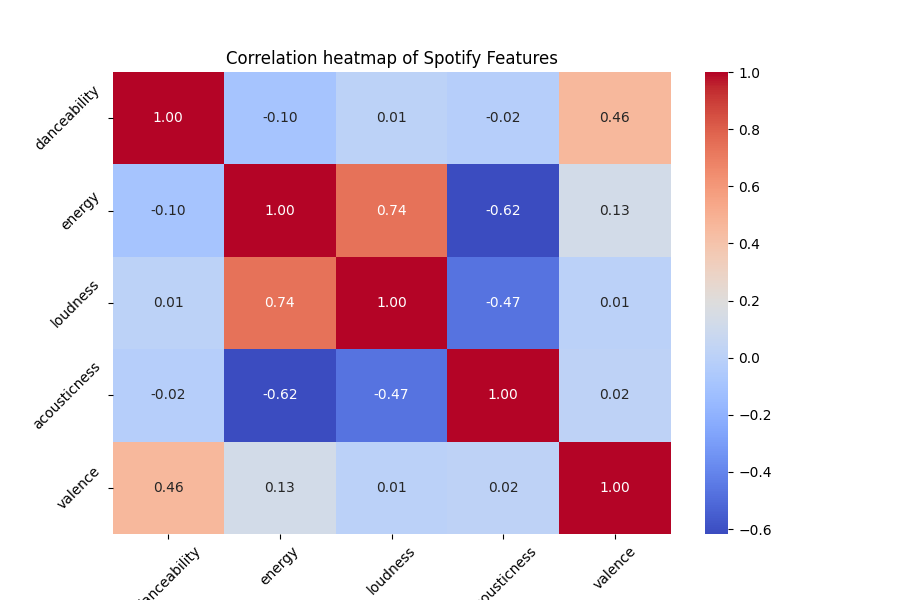
\includegraphics[width=6in]{img/corr_heatmap_spotify_features.png}
  \caption{Pearson's Correlation Heatmap of Spotify Features.}
  \label{Figure:corr_heatmap_spotify_features}
\end{figure}
\end{center}

\subsection*{Hierarchical Clustering}
\label{sec:hierarchicalclustering}

\begin{center}
\begin{figure}[H]
  \centering
  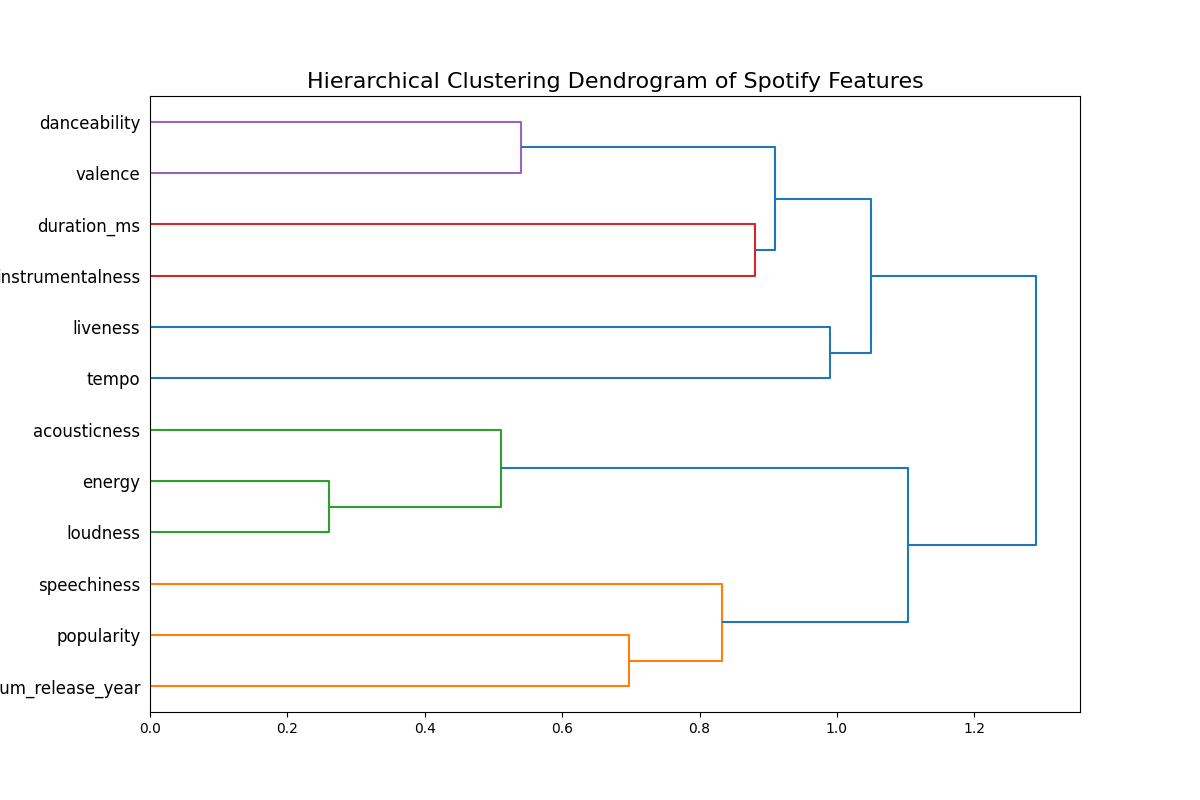
\includegraphics[width=6in]{img/dendrogram_spotify_features.png}
  \caption{Hierarchical Clustering of Spotify Features.}
  \label{Figure:dendrogram_spotify_features}
\end{figure}
\end{center}

\subsection*{Observations}
As shown on fig.~\ref{Figure:corr_heatmap_spotify_features} and
fig.~\ref{Figure:dendrogram_spotify_features}, Spotify audio features show high
level of correlation between each other, especially:
\begin{itemize}
  \item \textit{Energy} and \textit{Loudness}: A high correlation (0.74) suggest
    that energetic songs are typically louder;
  \item \textit{Danceability} and \textit{Valence}: high correlation between
    them indicates that songs perceived as positive and happy are usually more
    danceable;
  \item \textit{Energy} and \textit{Acousticness}: there is a strong negative
    correlation between those features, suggesting that high-energy tracks are
    less likely to have acoustic elements;
  \item The dendrogram (fig.~\ref{Figure:dendrogram_spotify_features}) shows relations
    between features and allows us to compare which features correlate with
    each other. In addition to the relationships seen in the correlation
    heatmap, we observe that \textit{popularity} appears to have a weak
    correlation with \textit{release year} and \textit{speechiness}.

\end{itemize}


%---------------------------------------------------------------------------


\section{Lyrical Features}

\subsection*{Correlation Heatmap}
\label{sec:correlationheatmapsspotifyfeatures}

\begin{center}
\begin{figure}[H]
  \centering
  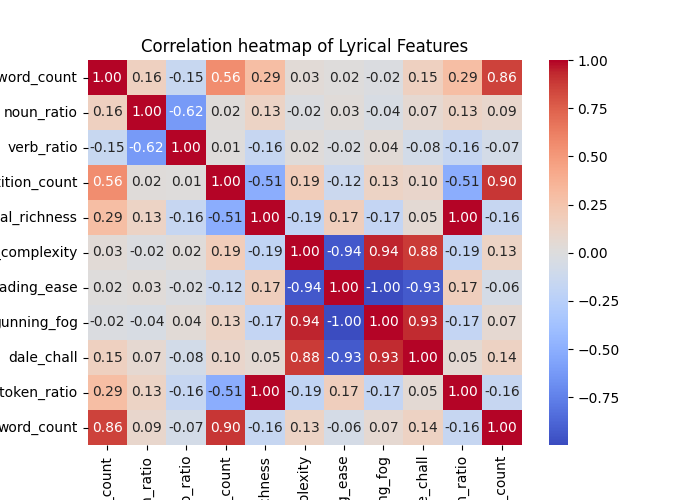
\includegraphics[width=6in]{img/corr_heatmap_lyrical.png}
  \caption{Pearson's Correlation Heatmap of Lyrical Features.}
  \label{Figure:corr_heatmap_lyrical}
\end{figure}
\end{center}

\subsection*{Hierarchical Clustering}
\label{sec:hierarchicalclustering}

\begin{center}
\begin{figure}[H]
  \centering
  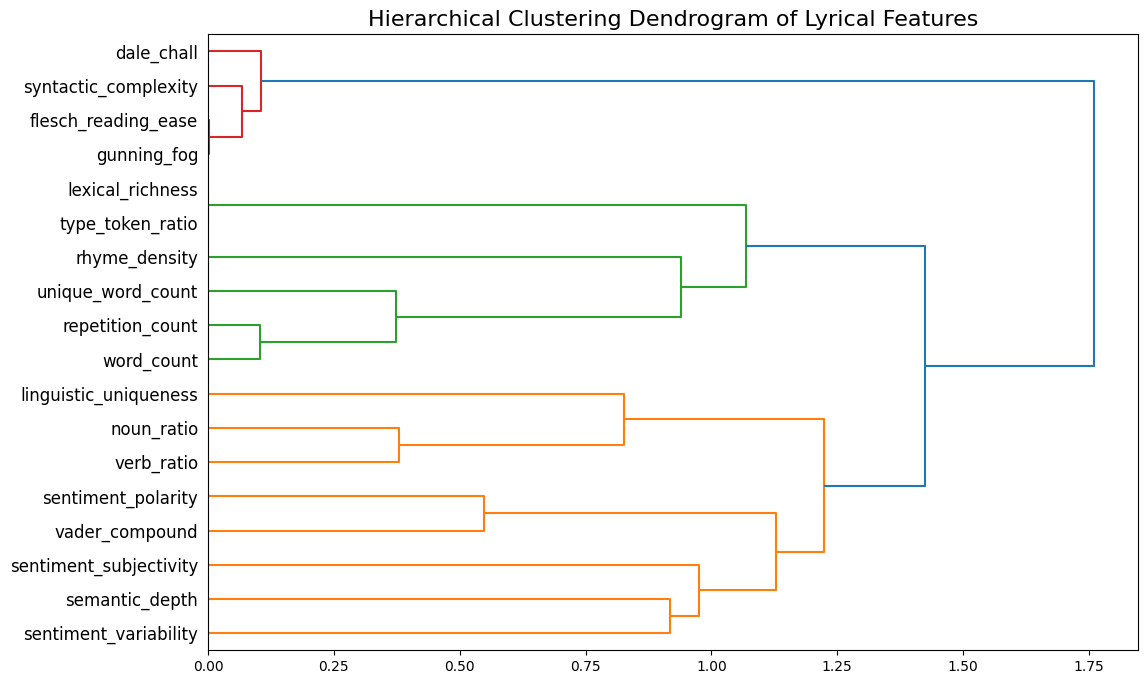
\includegraphics[width=6in]{img/dendrogram_lyrical.png}
  \caption{Hierarchical Clustering of Lyrical Features.}
  \label{Figure:dendrogram_lyrical}
\end{figure}
\end{center}


\subsection*{Observations}
Based on the figures fig.~\ref{Figure:corr_heatmap_lyrical} and
fig.~\ref{Figure:dendrogram_lyrical}, it can be observed that:
\begin{itemize}
  \item \textit{Flesch Reading Ease}, \textit{Gunning Fog} and \textit{Dale
    Chall} scores exhibit strong positive correlations, highlighting their
    shared focus on measuring lyrical complexity;
  \item \textit{Lexical Richness} correlates with \textit{Word Count},
    indicating that more lexically rich lyrics tend to have  greater variety
    of words;
  \item On the dendrogram we can distinguish three major clusters of features:
    \begin{itemize}
      \item \textbf{Lyrical Complexity Metrics} - \textit{Flesch Reading Ease},
        \textit{Gunning Fog}, \textit{Dale Chall} and \textit{Syntactic
        Complexity } quantify how difficult and complex the lyrics are;
      \item  \textbf{Lexical Features} - features such as \textit{Type-Token
        Ratio}, \textit{Lexical Richness} and \textit{Unique Word Count} form a
        cohesive cluster;
      \item \textbf{Sentiment-Related Features} - it includes \textit{Sentiment
        Polarity}, \textit{VADER Compound} and \textit{Semantic Depth}, which
        reflect emotional aspects of the lyrics.
    \end{itemize}
  \item Sentiment-related features are relatively closely grouped, suggesting a
    high level of interdependence.
\end{itemize}


%---------------------------------------------------------------------------
\section{Audio Features}

\subsection*{Correlation Heatmap}
\label{sec:correlationheatmapsspotifyfeatures}

\begin{center}
\begin{figure}[H]
  \centering
  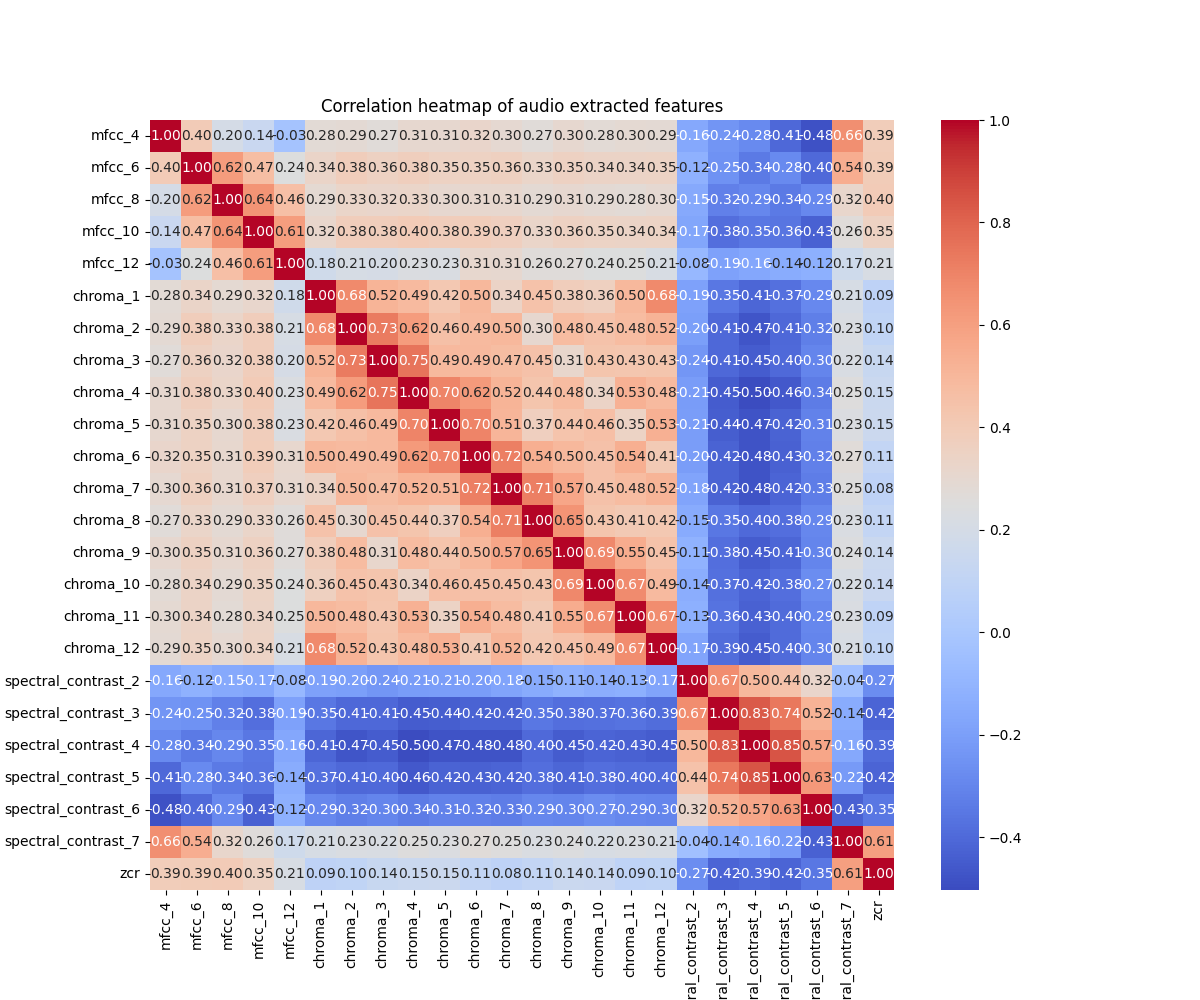
\includegraphics[width=6in]{img/corr_heatmap_audio.png}
  \caption{Pearson's Correlation Heatmap of Audio Features.}
  \label{Figure:corr_heatmap_audio}
\end{figure}
\end{center}

\subsection*{Hierarchical Clustering}
\label{sec:hierarchicalclustering}

\begin{center}
\begin{figure}[H]
  \centering
  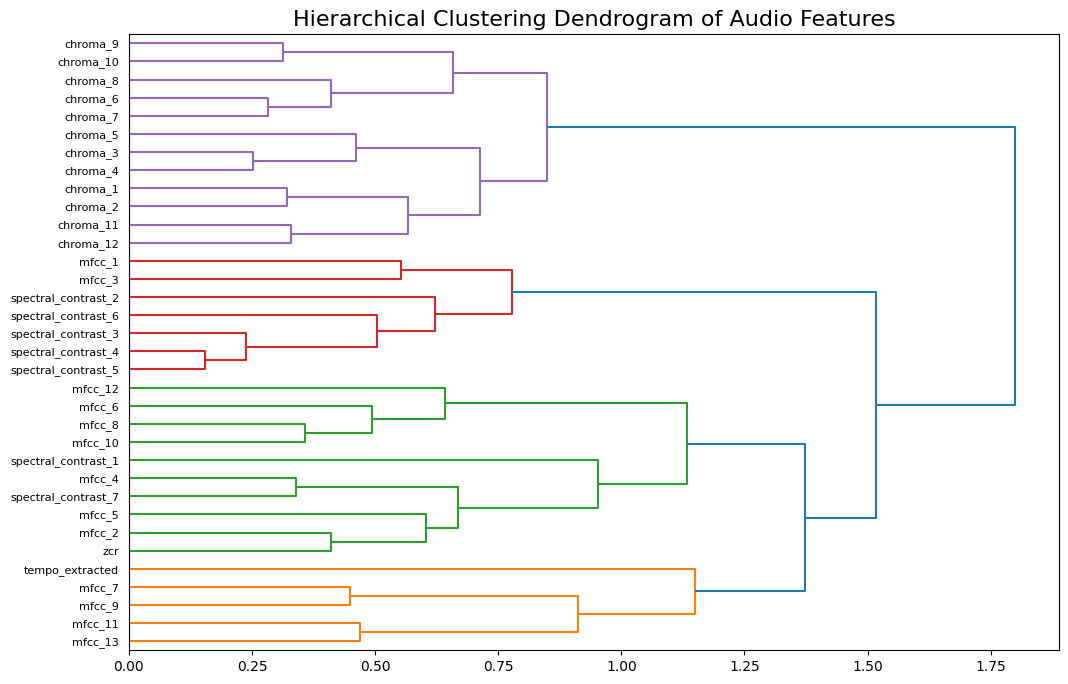
\includegraphics[width=6in]{img/dendrogram_audio.png}
  \caption{Hierarchical Clustering of Audio Features.}
  \label{Figure:dendrogram_audio}
\end{figure}
\end{center}


\subsection*{Observations}
The figures fig.~\ref{Figure:corr_heatmap_audio} and
fig.~\ref{Figure:dendrogram_audio} show that:
\begin{itemize}
  \item \textit{MFCC Features} are strongly correlated among themselves (e.g.
    \textit{mfcc\_4}, \textit{mfcc\_6}, \textit{mfcc\_8}, etc.);
  \item Similarily \textit{chroma} features show high correlation with each
    other, indicating that they capture similar aspects of audio tracks;
  \item \textit{spectral\_contrast} features show relatively small
    correlations with \textit{mfcc} and  \textit{chroma} features, indicating 
    their uniqueness;
  \item All \textit{chroma} features are grouped together in the same cluster
    on the dendrogram, supporting the conclusion drawn from the heatmap about
    strong correlations between them;
  \item \textit{zcr} and \textit{tempo\_extracted} are relatively independent;
  \item Some of the \textit{mfcc} and \textit{spectral\_contrast} features
    are to some degree correlated.
\end{itemize}

%---------------------------------------------------------------------------


\section{Empath Features}

\subsection*{Correlation Heatmap}
\label{sec:correlationheatmapsspotifyfeatures}

\begin{center}
\begin{figure}[H]
  \centering
  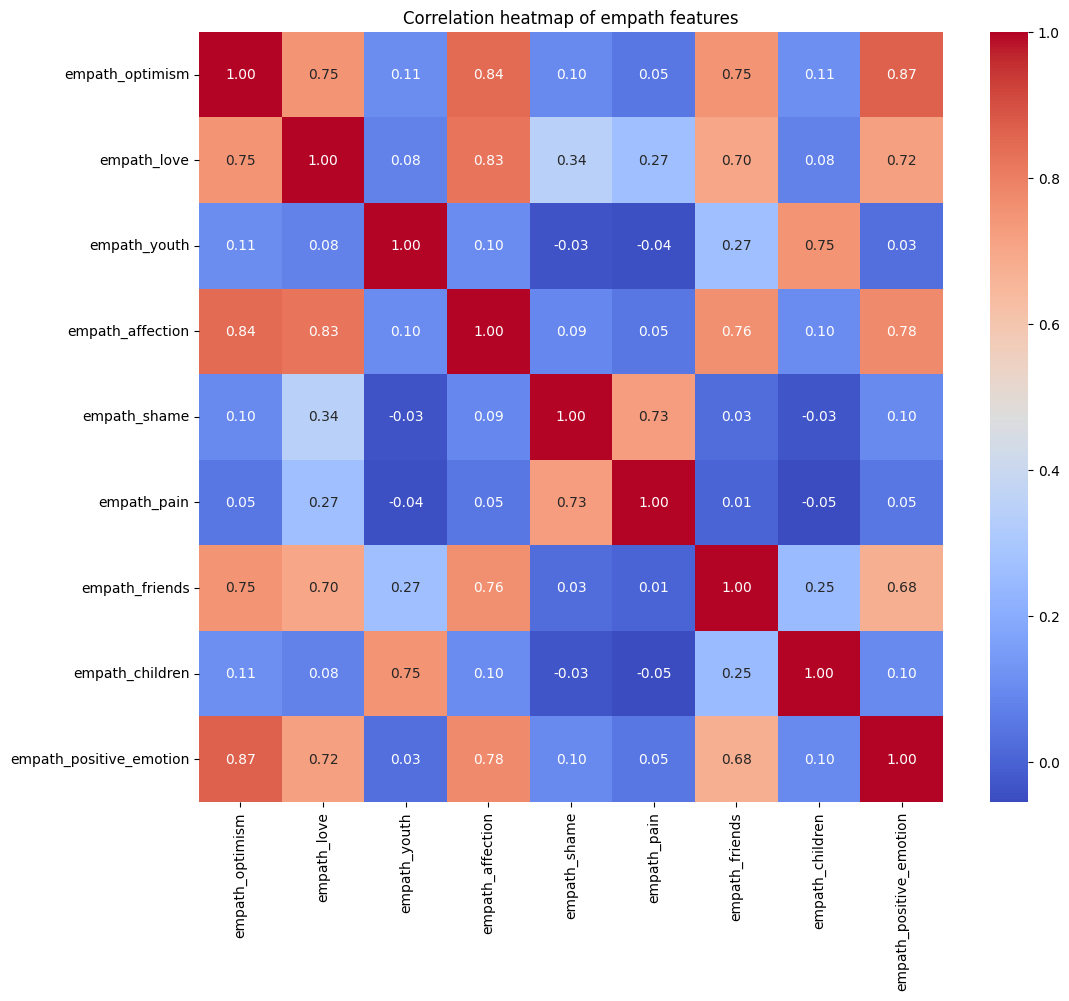
\includegraphics[width=6in]{img/corr_heatmap_empath.png}
  \caption{Pearson's Correlation Heatmap of Empath Features.}
  \label{Figure:corr_heatmap_empath}
\end{figure}
\end{center}

\subsection*{Hierarchical Clustering}
\label{sec:hierarchicalclustering}

\begin{center}
\begin{figure}[H]
  \centering
  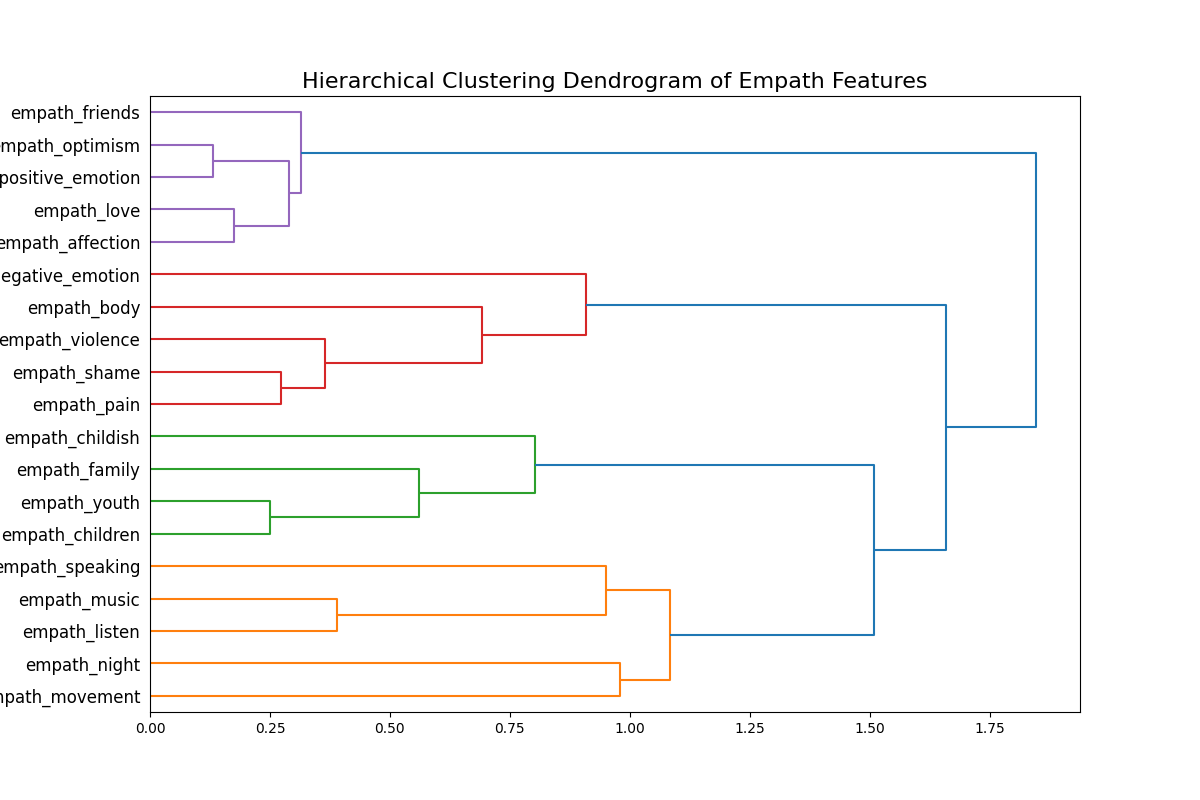
\includegraphics[width=6in]{img/dendrogram_empath.png}
  \caption{Hierarchical Clustering of Empath Features}
  \label{Figure:dendrogram_empath}
\end{figure}
\end{center}


\subsection*{Observations}
The correlation heatmap (fig.~\ref{Figure:corr_heatmap_empath}) and 
hierarchical clustering dendrogram (fig.~\ref{Figure:dendrogram_empath}) of
empath features provide the following information:
\begin{itemize}
  \item \textbf{High Correlations Reflect Logical Groupings}: high correlation
    between features like \textit{empath\_optimism}, \textit{empath\_love} and
    \textit{empath\_affection} align with the intuitive understanding that
    these aspects are closely related;
  \item Observed patters in correlations confirm that Empath was designed to
    group semantically related concepts together;
  \item The visualizations align with the intended design of Empath as a tool
    for interpretable feature extraction.
\end{itemize}


%---------------------------------------------------------------------------

\section{Genre Analysis}

\subsection{Genre Similarity}

\begin{center}
\begin{figure}[H]
  \centering
  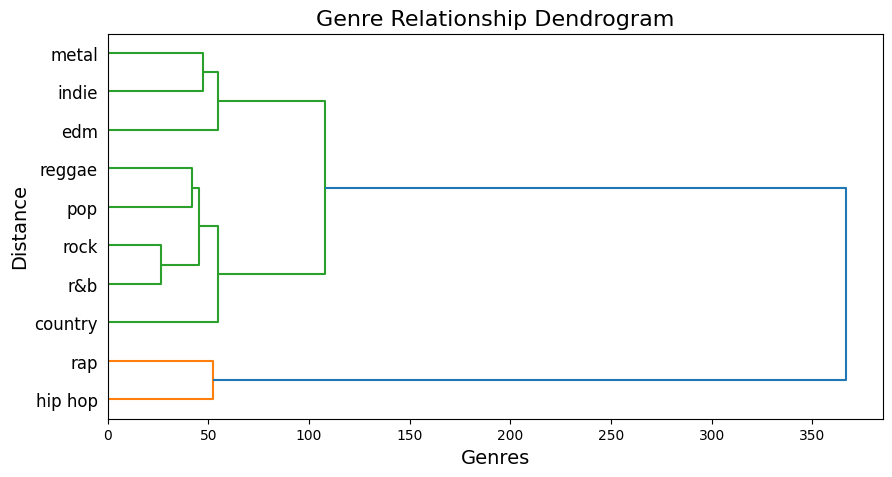
\includegraphics[width=6in]{img/genres_dendrogram.png}
  \caption{Hierarchical Clustering of Genres by lyrical and audio features.}
  \label{Figure:genres_dendrogram}
\end{figure}
\end{center}

\begin{center}
\begin{figure}[H]
  \centering
  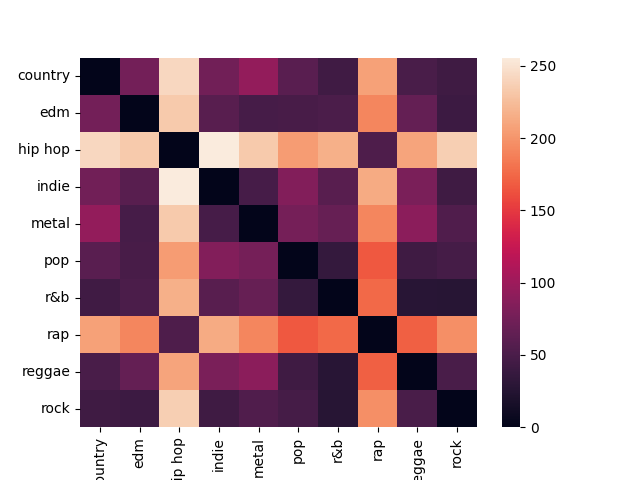
\includegraphics[width=6in]{img/genres_similarity_heatmap.png}
  \caption{Heatmap of euclidean distance of Genres calculated on lyrical and
  audio features.}
  \label{Figure:genres_similarity_heatmap}
\end{figure}
\end{center}

The dendrogram (fig.~\ref{Figure:genres_dendrogram}) illustrates hierarchical clustering of genres based on their
lyrical and audio features. The similarities between genres align with their
general cultural and musical understandings, e.g. rap and hip hop are closely
related, indicating that they're quite similar. 

The heatmap (fig.~\ref{Figure:genres_similarity_heatmap}) further supports this observation. The euclidean distances of rap
and hip hop with other genres stand out as the highest, meaning that those two
genres are similar to each other and very different to all other genres
included in this study. 

Interestingly, genres such as metal and indie, while
distinct in sound, share some overlap in features, which is reflected on the
dendrogram.


\begin{center}
\begin{figure}[H]
  \centering
  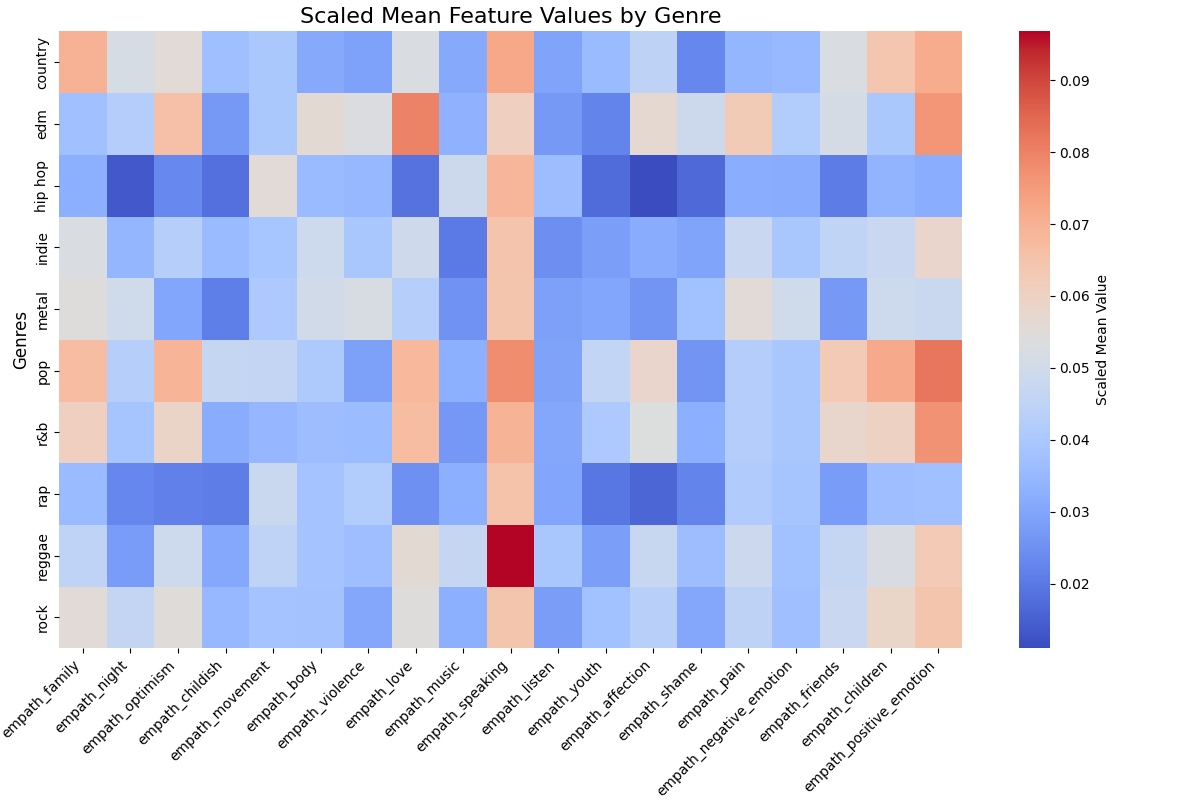
\includegraphics[width=6in]{img/heatmap_of_empath.png}
  \caption{Heatmap of mean values of empath features in each genre.}
  \label{Figure:heatmap_empath}
\end{figure}
\end{center}

The heatmap on figure fig.~\ref{Figure:heatmap_empath} displays scaled mean
values of \textit{Empath features} for different musical genres. It visualizes
the thematic  differences in their lyrics. It can be observed that:
\begin{itemize}
  \item \textbf{Country} music lyrics often involve topics related to family,
    love and  positive emotions. It seems to align well with genre's tendency
    to narrate personal, heartfelt and often nostalgic stories;
  \item \textbf{EDM} lyrics seem to often talk about love and optimism;
  \item For both \textbf{Hip Hop} and \textbf{Rap} according to Empath  the
    most prominent topic is \textit{speaking};
  \item For \textbf{Metal} high values in \textit{negative emotion} and
    \textit{pain} reflects the genre's focus on intense, darker themes;
  \item Higher values in \textit{love} and \textit{positive emotion}
    aligns with \textbf{Pop} music’s focus on themes of love and relationships;
  \item High values in \textit{friends} and \textit{optimism} categories
    reflect \textbf{Reggae's} focus on positivity, social connection, and
    uplifting messages.
\end{itemize}

\subsection{Lyrical Similarity Based on Embeddings}
\begin{center}
\begin{figure}[H]
  \centering
  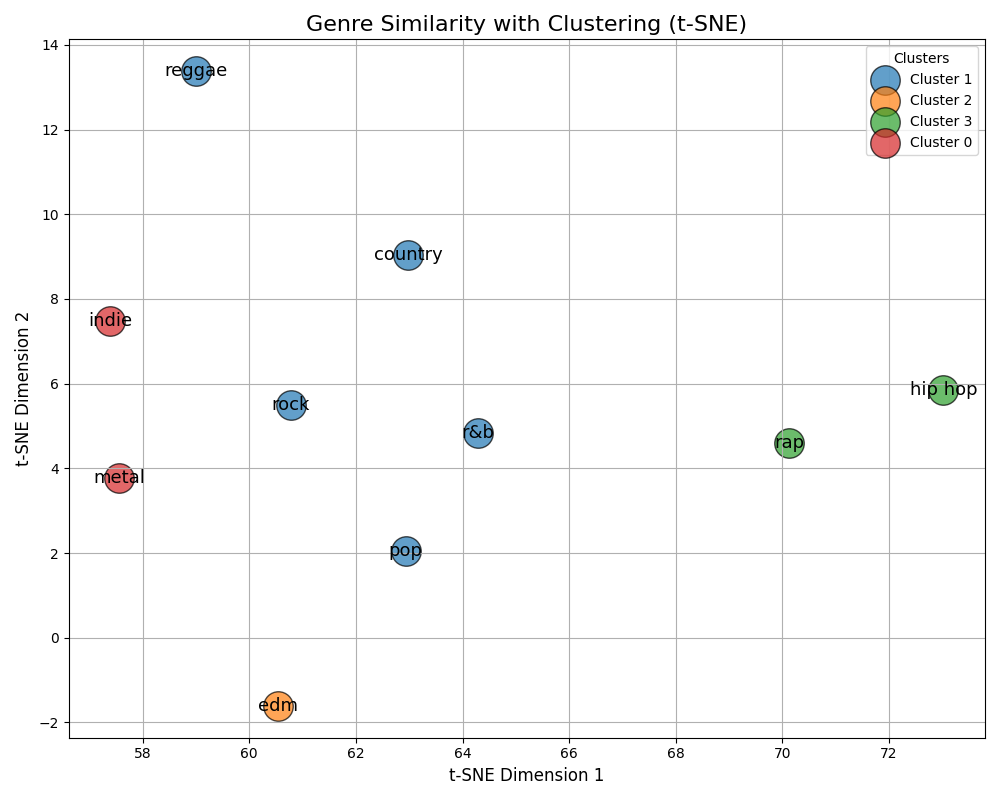
\includegraphics[width=6in]{img/tsne_genres.png}
  \caption{Lyrical Genre Similarity Based on Embeddings.}
  \label{Figure:tsne_genres}
\end{figure}
\end{center}
\textbf{t-SNE (t-Distributed Stochastic Neighbor Embedding)} is a statistical method for
visualizing high-dimensional data by reducing it to lower- dimensional spaces,
while preserving the relative distances and similarities between data points as
much as possible. It was applied to the euclidean distance matrix of mean
standardized Word2Vec and TF-IDF embeddings for each genre in order to
visualize lyrical similarities between different genres.

\textbf{K-means clustering} was applied as well on the mean standardized
embeddings per genre with near-optimal number of clusters determined using the
elbow method (which suggested four clusters). This operation clusters the most
similar genres together, additionally enhancing the visualization.


The resulting scatterplot (fig.~\ref{Figure:tsne_genres}) shows that:
\begin{itemize}
  \item \textit{Hip hop} and \textit{rap} form a distinct cluster, indicating
    strong lyrical and thematic similarity and dissimilarity with other genres;
  \item \textit{Reggae} is slightly separate from other genres but still
    belongs to the cluster that includes \textit{rock}, \textit{pop},
    \textit{country}, and \textit{R\&B}, suggesting moderate similarity in
    lyrical and thematic content of songs belonging to those genres;
  \item \textit{Metal} and \textit{indie} are closely positioned, sharing
    overlapping themes and forming a  separate cluster;
  \item \textit{EDM} is positioned furthest from other genres and belongs to
    its own cluster, highlighting its unique lyrical and thematic style.
\end{itemize}

\subsection{Top Genre Characteristics}
\begin{center}
\begin{figure}[H]
  \centering
  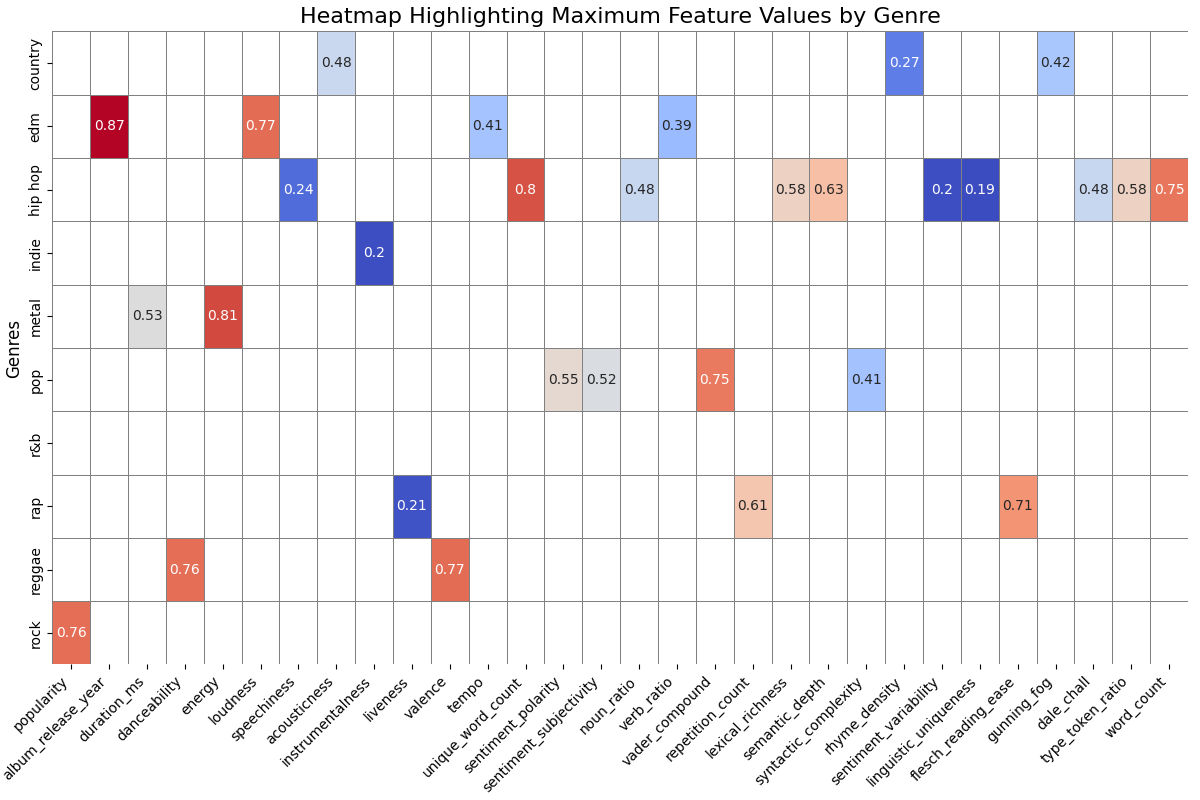
\includegraphics[width=6in]{img/heatmap_max_feature_values_by_genre.png}
  \caption{Heatmap highlighting the maximum feature values across genres.}
  \label{Figure:heatmap_max_feature_values_by_genre}
\end{figure}
\end{center}
On the figure fig.~\ref{Figure:heatmap_max_feature_values_by_genre} each filled
cell represents the genre that exhibits the highest mean value for the
corresponding feature, calculated using scaled feature values. This
visualization emphasizes distinctive characteristics of each genre, and allows
to see ``in  which genre the feature achieved its highest mean''.

\begin{itemize}
  \item \textbf{Country}: Highest in acousticness and rhyme density;
  \item \textbf{EDM}: Dominated in tempo, loudness, and featured the most
    recent songs;
  \item \textbf{Hip Hop}: Excelled in unique word count, lexical richness, and
    semantic depth;
  \item \textbf{Metal}: Stood out for energy and longer song durations;
  \item \textbf{Pop}: Showed the highest positivity (VADER compound) and
    subjectivity in lyrics;
  \item \textbf{Rap}: Highest in repetition count and reading ease;
  \item \textbf{Reggae}: Highlighted by high valence and danceability;
  \item \textbf{Rock}: Scored highest in in popularity.
    
\end{itemize}

\begin{center}
\begin{figure}[H]
  \centering
  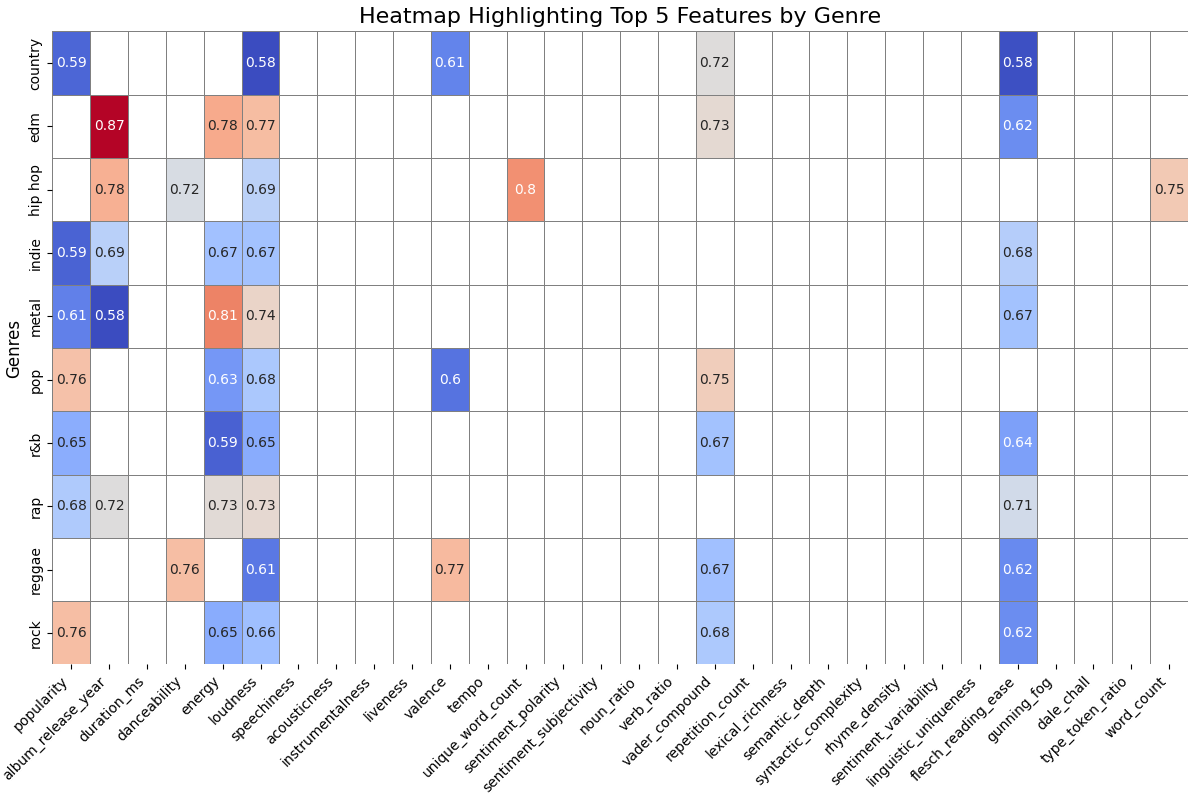
\includegraphics[width=6in]{img/heatmap_top_feature_values_by_genre.png}
  \caption{Heatmap highlighting the top 5 features by genre. Each filled cell
    represents one of the five highest mean feature values for a given genre,
    calculated on scaled data. This visualization shows what are ``the top 5
    most characteristic properties of each genre''. }
  \label{Figure:heatmap_top_feature_values_by_genre}
\end{figure}
\end{center}

Lastly, we switch perspectives, focusing not on individual features but instead
examining each genre to identify the top 5 features that characterize it. Each
filled cell on the resulting
heatmap (fig.~\ref{Figure:heatmap_top_feature_values_by_genre}) shows one of the
five most prominent characteristics exhibited by that genre.


\chapter{Experiments and Results}
\label{cha:experimentsandresults}
%---------------------------------------------------------------------------

\section{Song Popularity}
\label{sec:songpopularity}

The analysis of song popularity provides valuable insights into the factors
that influence the success of music tracks. This problem has two approaches:
\begin{itemize}
  \item \textbf{Regression} - Spotify's popularity is a value on scale of
    0-100. This approach involves training a regression model trying to predict
    that value.
  \item \textbf{Classification} - assigning binary label to the songs(popular
    vs. unpopular) and training a classification model to predict it.
\end{itemize}

In this section the prediction of popularity was attempted using several
regression and classification models. These models were trained on different
sets of features, including Spotify metadata, lyrical attributes, and audio
features, with the aim of investigating the predictive power of those features
and their impact on popularity.

Catboost models were used as the primary predictive tool due to their
robustness and performance in handling complex relationships. 

Baseline models were also implemented to serve as a reference point:
\begin{itemize}
  \item \textit{Baseline Mean Model}: baseline model for regression that always predicts the mean.
  \item \textit{Baseline Majority Model}: baseline model for classification that always predicts the majority class.
  \item \textit{Baseline Random Model}: baseline model for classification that predicts random class.
\end{itemize}

The experiments involved both quantitative evaluatoin and SHAP analysis to
assess feature importance and interpretability of the models.

\subsection{Regression Approach}

\begin{center}
\begin{figure}[H]
  \centering
  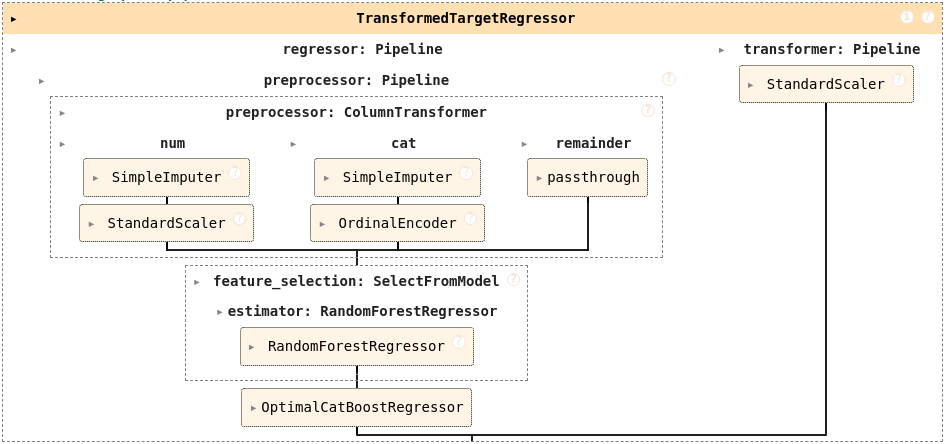
\includegraphics[width=6in]{img/reg_pipeline.png}
  \caption{Regression model pipeline. It involves preprocessing, feature
  selection and CatBoost model.}
  \label{Figure:fig_beh}
\end{figure}
\end{center}

The pipeline was fit with all available features, that includes Spotify audio
features and metadata, lyrical features and features extracted from the audio
files. The feature selection step chose the subset of most valuable features
based on the feature importance from initial Random Forest model.

% \usepackage{tabularray}
\begin{table}[H]
\centering
\caption{Results of regression of popularity.}
\begin{tblr}{
  hline{2} = {-}{},
}
 & \textbf{Model}      & \textbf{Features} & \textbf{MAE}  & \textbf{RMSE} & $R^2$         \\
 & Baseline Mean Model &                   & 13.53         & 16.90         & -0.01         \\
 & Catboost            & all               & \textbf{6.14} & \textbf{8.35} & \textbf{0.75} \\
 & Catboost            & lyrical           & 11.90         & 15.30         & 0.17          \\
 & Catboost            & spotify data      & 6.26          & 8.49          & 0.74          \\
 & Catboost            & audio             & 12.77         & 16.19         & 0.07          
\end{tblr}
\end{table}

As seen in the results table, the CatBoost model with all features achieved the
best performance, with \textbf{Mean Absolute Error(MAE) of \textbf{6.14} and
$R^2$ of 0.75}, closely followed by the model trained only on spotify metadata
and audio features. That observation shows that the spotify data offers  best
features for the task of predicting song popularity. In comparison to the
\textit{Baseline Mean Model}, the best model reduced MAE by \textbf{54.6\%} and
demonstrated a very high $R^2$.


SHAP analysis was conducted to interpret the predictions of the regression
model and asses the importance of individual features and their contribution to
song's popularity.


\begin{center}
\begin{figure}[H]
  \centering
  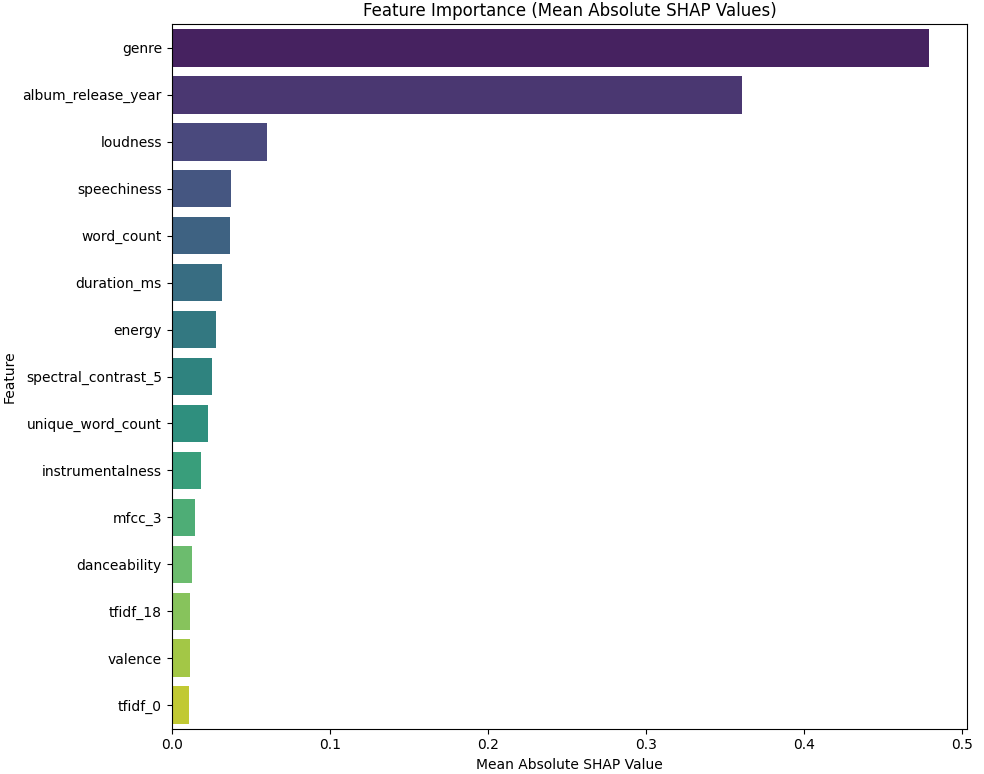
\includegraphics[width=5in]{img/feature_importance_popularity_reg.png}
  \caption{SHAP feature importance plot of the regression model for popularity.}
  \label{Figure:fig_beh}
\end{figure}
\end{center}


The mean absolute SHAP values were used to rank the overall importance of input
features. Key insights:
\begin{itemize}
  \item \textbf{Dominance of \textit{Genre} and \textit{Album Release Year}.}:
    these two features account for the majority of the predictive power in the
    model. Genre captures the musical style and release year reflects trends
    and cultural preferences over time.
  \item Spotify's audio features like \textit{loudness} and
    \textit{speachiness} showed moderate contribution to model's performance.
    Their score highlights their relevance in describing popular tracks' audio
    characteristics.
  \item Lyric-based features like \textit{word count} and \textit{unique word
    count} were significantly less impactful, however still contributed to
    model's performance to some degree.
\end{itemize}

\begin{center}
\begin{figure}[H]
  \centering
  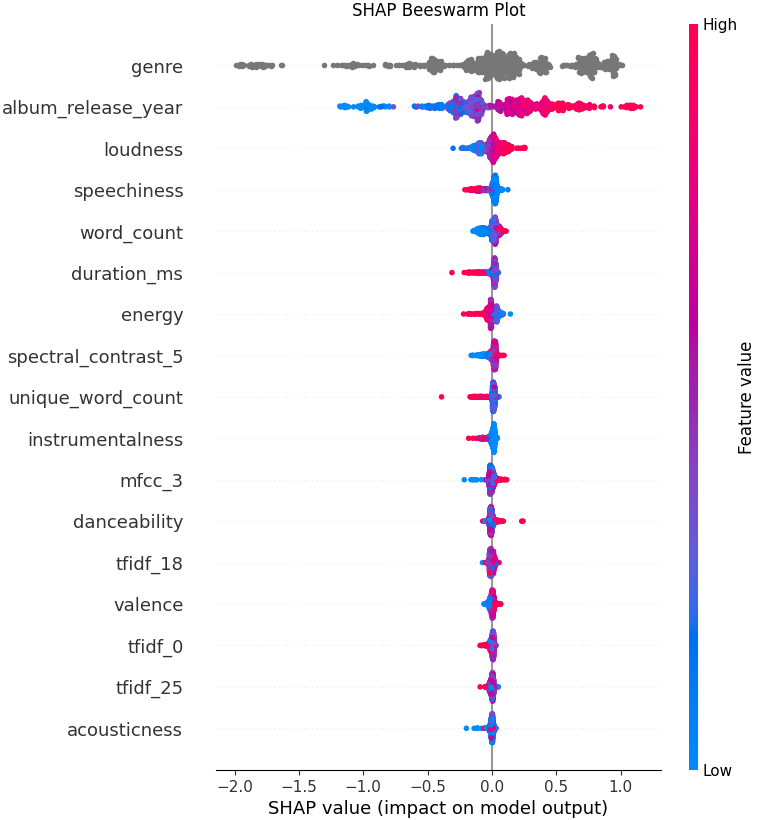
\includegraphics[width=5in]{img/beeswarm_popularity_reg.png}
  \caption{SHAP beeswarm plot of the regression model for popularity.}
  \label{Figure:fig_beh}
\end{figure}
\end{center}

\begin{itemize}
  \item Higher values of \textit{Release Year} usually result in higher
    \textit{Popularity}, which indicates that newer songs are usually more
    popular.
  \item Higher \textit{loudness} and certain levels of \textit{speechiness}
    positively correlate with higher \textit{popularity} in many cases,
    reflecting their impact on listener preferences.
\end{itemize}



\subsection{Classification Approach}

The task of predicting song popularity was reformulated as a binary
classification problem, where the target was to determine whether a song is
"popular" (1) or "not popular" (0). In order to create those labels from an
integer variable with range 0-100, the \textbf{70th perrcentile of the
popularity values was used as the threshold}. Songs with popularity greater or
equal  than this  threshold werre  labeled as popular, and the rest was labeled
as unpopular. This thresholding approach based on quantile ensures a balanced
representation of popular songs in the dataset while accounting for the
naturally skewed distribution of  popularity scores.



% \usepackage{tabularray}
\begin{table}[H]
\centering
\caption{Results of classification of popularity.}
\begin{tblr}{
  hline{2} = {-}{},
}
 & \textbf{Model}          & \textbf{Features} & \textbf{Accuracy} & \textbf{F1(w.avg.)} \\
 & Baseline Majority Model &                   & 62.90\%           & 48.57\%             \\
 & Baseline Random Model   &                   & 52.55\%           & 53.34\%             \\
 & Catboost                & all               & \textbf{84.13\%}  & \textbf{84.13\%}    \\
 & Catboost                & lyrical           & 66.75\%           & 66.25\%             \\
 & Catboost                & spotify data      & \textbf{84.41\%}  & \textbf{84.63\%}    \\
 & Catboost                & audio             & 64.55\%           & 63.73\%             
\end{tblr}
\end{table}

The classification models were evaluated using accuracy and weighted F1-score.
\textit{Baseline Majority Model} (which predicts the majority class for all samples)
achieved an accuracy of 62.90\% and an F1-score of 48.57\%. This reflects the
class imbalance introduced by the thresholding, with a higher proportion of
songs being labeled as "not popular."

The Baseline Random Model, which randomly guesses classes, performed worse than
the majority baseline in terms of accuracy (52.55\%) but achieved a slightly
higher F1-score (53.34\%) due to the randomness capturing some minority class
predictions correctly.

The CatBoost model significantly outperformed both baselines, achieving an
overall accuracy of 84.13\% and a weighted F1-score of 84.13\% trained on all
features.

CatBoost trained on Spotify data managed to slightly outperform the model
trained on all features, further reinforcing the observation that Spotify audio
features and metadata are the strongest predictors of popularity.

The model using only lyrical features showed relatively lower performance, with
an accuracy of 66.75\% and an F1-score of 66.25\%. This indicates that while
lyrics contribute to song popularity, they are far less predictive than other
feature sets.

The performance of the model trained on features extracted from audio files was
similar to the lyrical one, demonstrating that isolated audio features are not
suffficient to fully predict popularity.


SHAP analysis was conducted to understand the feature dependencies and
importance for the classification task. As expected, the results were
consistent with the regression analysis of popularity. Key features such as
\textit{genre}, \textit{album release year}, \textit{danceability}, and \textit{loudness} emerged as the most
significant predictors, mirroring their importance in the regression task. This
consistency underscores the robustness of these features in modeling song
popularity across different approaches (regression and classification).

\begin{center}
\begin{figure}[H]
  \centering
  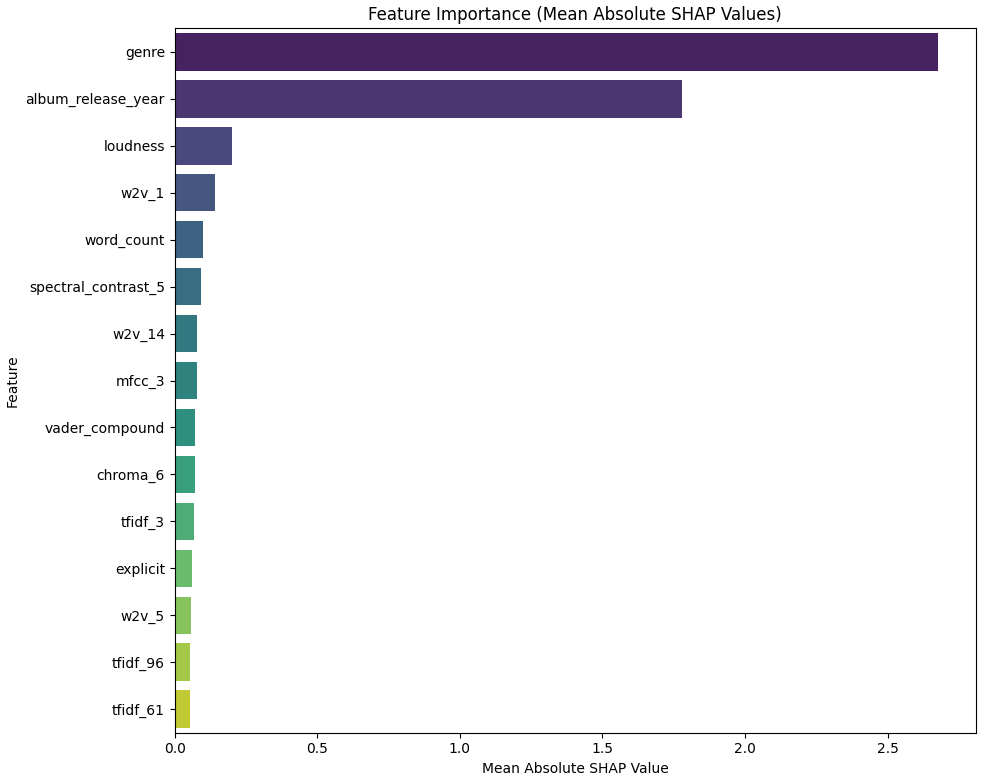
\includegraphics[width=5in]{img/feature_importance_popularity_clf.png}
  \caption{SHAP feature importance plot of the classification model for popularity.}
  \label{Figure:fig_beh}
\end{figure}
\end{center}

\begin{center}
\begin{figure}[H]
  \centering
  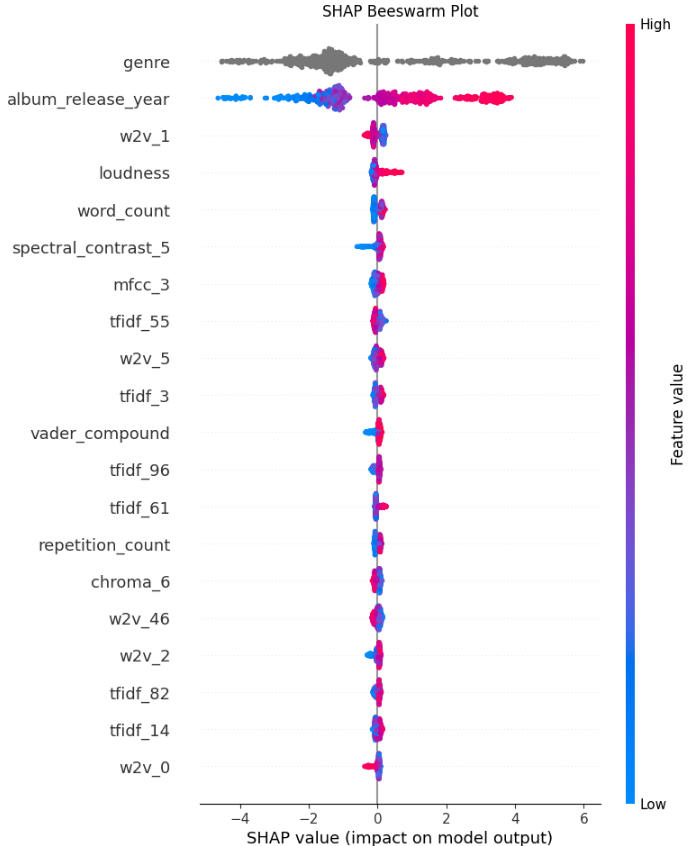
\includegraphics[width=5in]{img/beeswarm_popularity_clf.png}
  \caption{SHAP beeswarm plot of the classification model for popularity.}
  \label{Figure:fig_beh}
\end{figure}
\end{center}



The SHAP analysis for the classification model highlights similar dependencies
to the regression model. Key features like \textit{genre} and
\textit{album release year} remain the most important, emphasizing their role
in shaping song popularity. 

Several differences can be observed between feature importance in the
regression and classification model, notably:
\begin{itemize}
  \item Lyrics embeddings(TF-IDF and Word2Vec) seemed to play a bigger role in
    the classification model.
  \item Classification model seemed to pay much less attention to Spotify audio
    features, like \textit{danceability}, \textit{energy} and
    \textit{speechiness}.
  \item Unlike in regression, in classification a sentiment metric,
    \textit{VADER compound} contributed to the prediction of popularity. More
    popular songs tend to have more positive lyrics.
\end{itemize}

\section{Explicitness}
\label{sec:explicitness}

The task of predicting whether a song contains explicit content was approached
as a classification problem. The performance of the CatBoost model was compared
against baseline on different feature subsets. One of the key challenges of
this problem was significant class imbalance present in the dataset;
approximately 85\% of the songs did not contain explicit content.

Significant class imbalance can lead to models favoring the majority class,
potentially resulting in  high accuracy but poor performance on the minority
class. To address this problem, CatBoost's class weights parameter was used.
This parameter allowed the model to penalize misclassifications of the minority
class more heavily, therefore improving its ability to recognize explicit
content.

% \usepackage{tabularray}
\begin{table}[H]
\centering
\caption{Results of classification of explicitness.}
\begin{tblr}{
  hline{2} = {-}{},
}
 & \textbf{Model}          & \textbf{Features} & \textbf{Accuracy} & \textbf{F1 weighted average} \\
 & Baseline Majority Model &                   & 84.00\%           & 76.69\%                      \\
 & Baseline Random Model   &                   & 50.06\%           & 56.57\%                      \\
 & Catboost                & all               & \textbf{92.68\%}  & \textbf{92.72\%}             \\
 & Catboost                & lyrical           & \textbf{92.55\%}  & \textbf{92.41\%}             \\
 & Catboost                & spotify data      & 85.93\%           & 86.41\%                      \\
 & Catboost                & audio             & 84.13\%           & 83.03\%                      
\end{tblr}
\end{table}

The table presents the results of the models in terms of accurracy and weighted
F1 score. The \textit{Baseline Majority Model} achieved accuracy of 84\% and
significantly lower F1 weighted average of 76.69\%, which reflects its inability
to handle class balance effectively. The \textit{Baseline Random Model}
performed very poorly, with an accuracy of 50.06\% and F1 weighted average of
56.57\%.

In contrast, the CatBoost model outperformed both baselines achieving accuracy
of \textbf{92.68\%} and weighted average score of \textbf{92.72\%} when trained
on all features. Interestingly, the model trained only using lyrical features
performed nearly as well, indicating that explicitness can larrgely be
predicted based on lyrrical content. Models that relied on Spotify metadata and
features extracted from audio files had lower performance, achieving accurracy
close to \textit{Baseline Majority Model}, but with higher F1 scores. This
observation emphasizes the centrality of lyrical information in prediction of
explicit content.


\begin{center}
\begin{figure}[H]
  \centering
  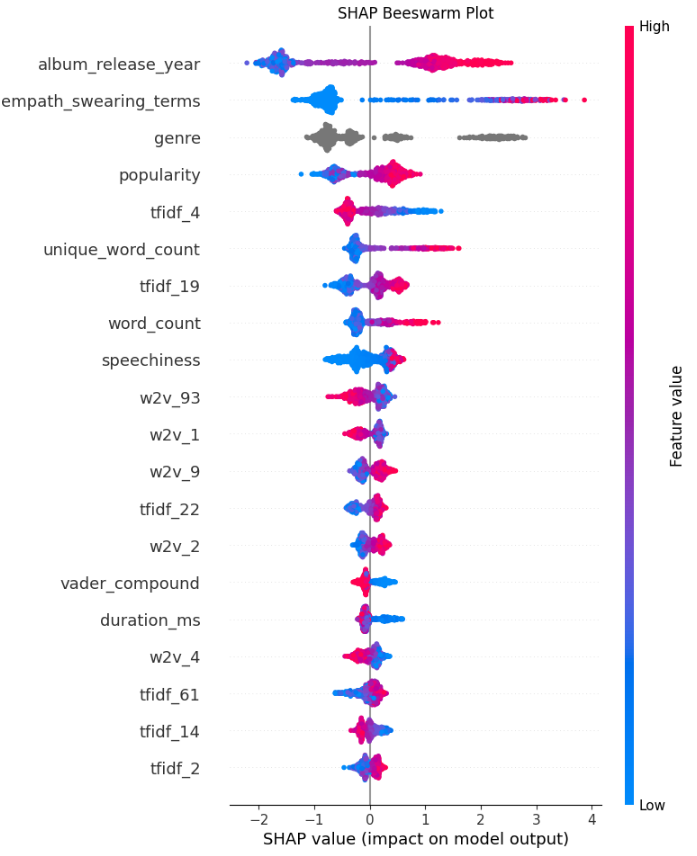
\includegraphics[width=5in]{img/beeswarm_explicitness.png}
  \caption{SHAP beeswarm plot of the classification model for explicitness.}
  \label{Figure:fig_beh}
\end{figure}
\end{center}

\begin{center}
\begin{figure}[H]
  \centering
  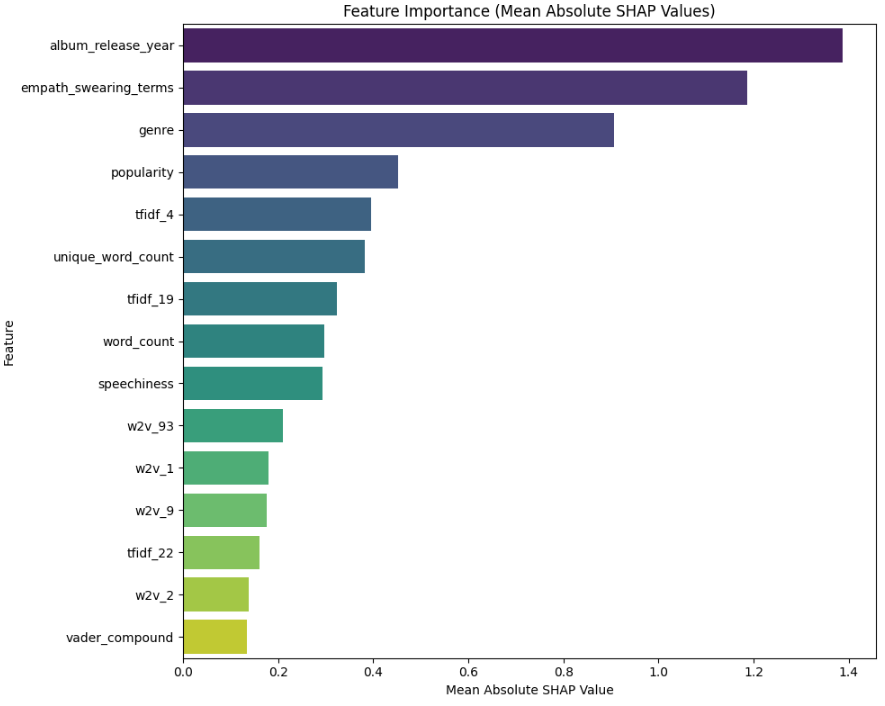
\includegraphics[width=5in]{img/feature_importance_explicitness.png}
  \caption{SHAP beeswarm plot of the classification model for explicitness.}
  \label{Figure:fig_beh}
\end{figure}
\end{center}


Key features for this task turned out to be:
\begin{itemize}
  \item \textbf{Album Release Year}: this feature had  highest feature
    importance, reflecting temporal trends in explicit content. Newer songs are
    statistically more likely to contain explicit language, reflecting changing
    societal norms and artistic expressions over time.
  \item \textbf{Empath Swearing Terms}: As expected, the presence of swearing
    terms was a strong indicator of explicitness.
  \item \textbf{Genre} was the third most important feature, showing that
    certain genres  are more likely to contain explicit content than others.
  \item \textbf{TF-IDF}: several vectors created using TF-IDF and later reduced
    via PCA significantly contributed to the model's predictions. Similar to
    the Empath feature, TF-IDF likely captured swear words and related patterns
    in the lyrics, reinforcing its importance.
  \item \textbf{Speechiness}: songs with higher values of
    speechiness—indicating a greater presence of spoken-word elements—were more
    likely to be labeled as explicit.
\end{itemize}

\chapter{Conclusion and Future Work}
\label{cha:conclusionandfuturework}
%---------------------------------------------------------------------------

\section{Summary of Contributions}
\label{sec:summaryofcontributions}


%---------------------------------------------------------------------------

\section{Recommendations for Future Work}
\label{sec:recommendationsforfuturework}


% \include{rozdzial8}
% \include{rozdzial9}

\cleardoublepage % Dodaj nową stronę, aby "Literatura" zaczęła się na nieparzystej stronie
\phantomsection % Dodaj punkt w spisie treści dla sekcji "Literatura"
\addcontentsline{toc}{chapter}{Bibliography} % Dodaj "Literatura" do spisu treści, bez numerowania
\printbibliography[title={Bibliography}]
\end{document}
